\documentclass{beamer}

\usepackage[UTF8]{ctex}
\usepackage{graphicx}
\usepackage{booktabs}
\usepackage{amsmath}

% ===== 更新slides时注意终端bash输入 =====
% git add .
% git commit -m "update: event study figure"
% git commit -m "add: background slide"
%git commit -m "add: intensive margin slide"
% 修改版本：
%git tag -a v1.4-2026-04-27 -m "intensive margin completed"
%git push origin --tags


% git push

% ===== 极简风格 =====
\usetheme{default}
\usecolortheme{default}
\setbeamertemplate{navigation symbols}{} % 去掉右下角按钮
\setbeamertemplate{footline}[frame number] % 只保留页码

% 标题信息
\title{Pharmaceutical Reform and Pharmacy Entry: Evidence from Hospitals in China}
\author{Wenxia Chen}
\date{April ,2026}

\begin{document}



% ================= 标题页 =================


\frame{\titlepage}

% ================= 研究背景 =================
\begin{frame}{Institutional Background}

China's pharmaceutical reform aims to eliminate the long-standing 
“drug mark-up” mechanism in public hospitals.

\begin{itemize}
    \item \textbf{Financing Reform:}
    Public hospitals previously relied on three revenue sources:
    service fees, drug mark-ups, and government subsidies. 
    The reform removes drug mark-ups, shifting the system to a 
    two-channel structure: service fees and government subsidies.

    \item \textbf{Price Adjustment:}
    The policy eliminates drug mark-ups while increasing the prices 
    of medical services, including consultation, surgery, and nursing, 
    to better reflect the value of medical labor.

    \item \textbf{Complementary Policies:}
    The reform is accompanied by changes in health insurance payment 
    methods and strengthened government responsibility in hospital financing.
\end{itemize}

\end{frame}

\begin{frame}{Reform Rollout and Scope}


The reform was first implemented as a pilot program targeting county-level public hospitals. It introduced a comprehensive set of changes, including reforms to hospital governance, financing mechanisms, personnel and compensation systems, drug procurement and supply, as well as the medical pricing system.
 \begin{itemize}
 \item The pilot was launched in 2012 and covered approximately 300 counties (or county-level cities).

 \item Following the pilot phase, the reform was gradually expanded nationwide and was fully implemented by the end of September 2017. All public hospitals adopted the reform, with a universal removal of drug mark-ups, except for traditional Chinese medicine herbal decoctions.

\item{The staggered rollout of the reform provides quasi-experimental variation for empirical analysis.}
\end{itemize}

\end{frame}

\begin{frame}{Distribution of Policy Adoption Years}

\centering
\footnotesize

\begin{tabular}{lccc}
\hline
\hline
Policy Year & Frequency & Percent (\%) & Cumulative (\%) \\
\hline
Never treated (private hospitals) & 86,027 & 34.37 & 34.37 \\
2012 & 6,494 & 2.59 & 36.97 \\
2013 & 1,620 & 0.65 & 37.62 \\
2014 & 34,471 & 13.77 & 51.39 \\
2015 & 43,131 & 17.23 & 68.62 \\
2016 & 16,619 & 6.64 & 75.26 \\
2017 & 61,904 & 24.74 & 100.00 \\
\hline
Total & 250,266 & 100.00 & \\
\hline
\hline
\end{tabular}

\end{frame}

% ================= 文献综述部分 =================

% ================= 数据 =================
\begin{frame}{Data Sources}

\textbf{Hospital Data.} Information on hospitals is obtained from business registration records, including hospital name, classification (level), industry code, province, county, and geographic coordinates.

\medskip

\textbf{Pharmacy Data.} Pharmacy data are collected from Dianping, including merchant name, industry classification, geographic coordinates, and an indicator for chain affiliation.

\medskip

\textbf{Reform Data.} Information on the timing and implementation of the reform is compiled from official government policy documents and related reports.

\end{frame}



\begin{frame}{Distribution of Pharmacy Density Around Hospitals}

\centering

\begin{minipage}{0.32\textwidth}
\centering
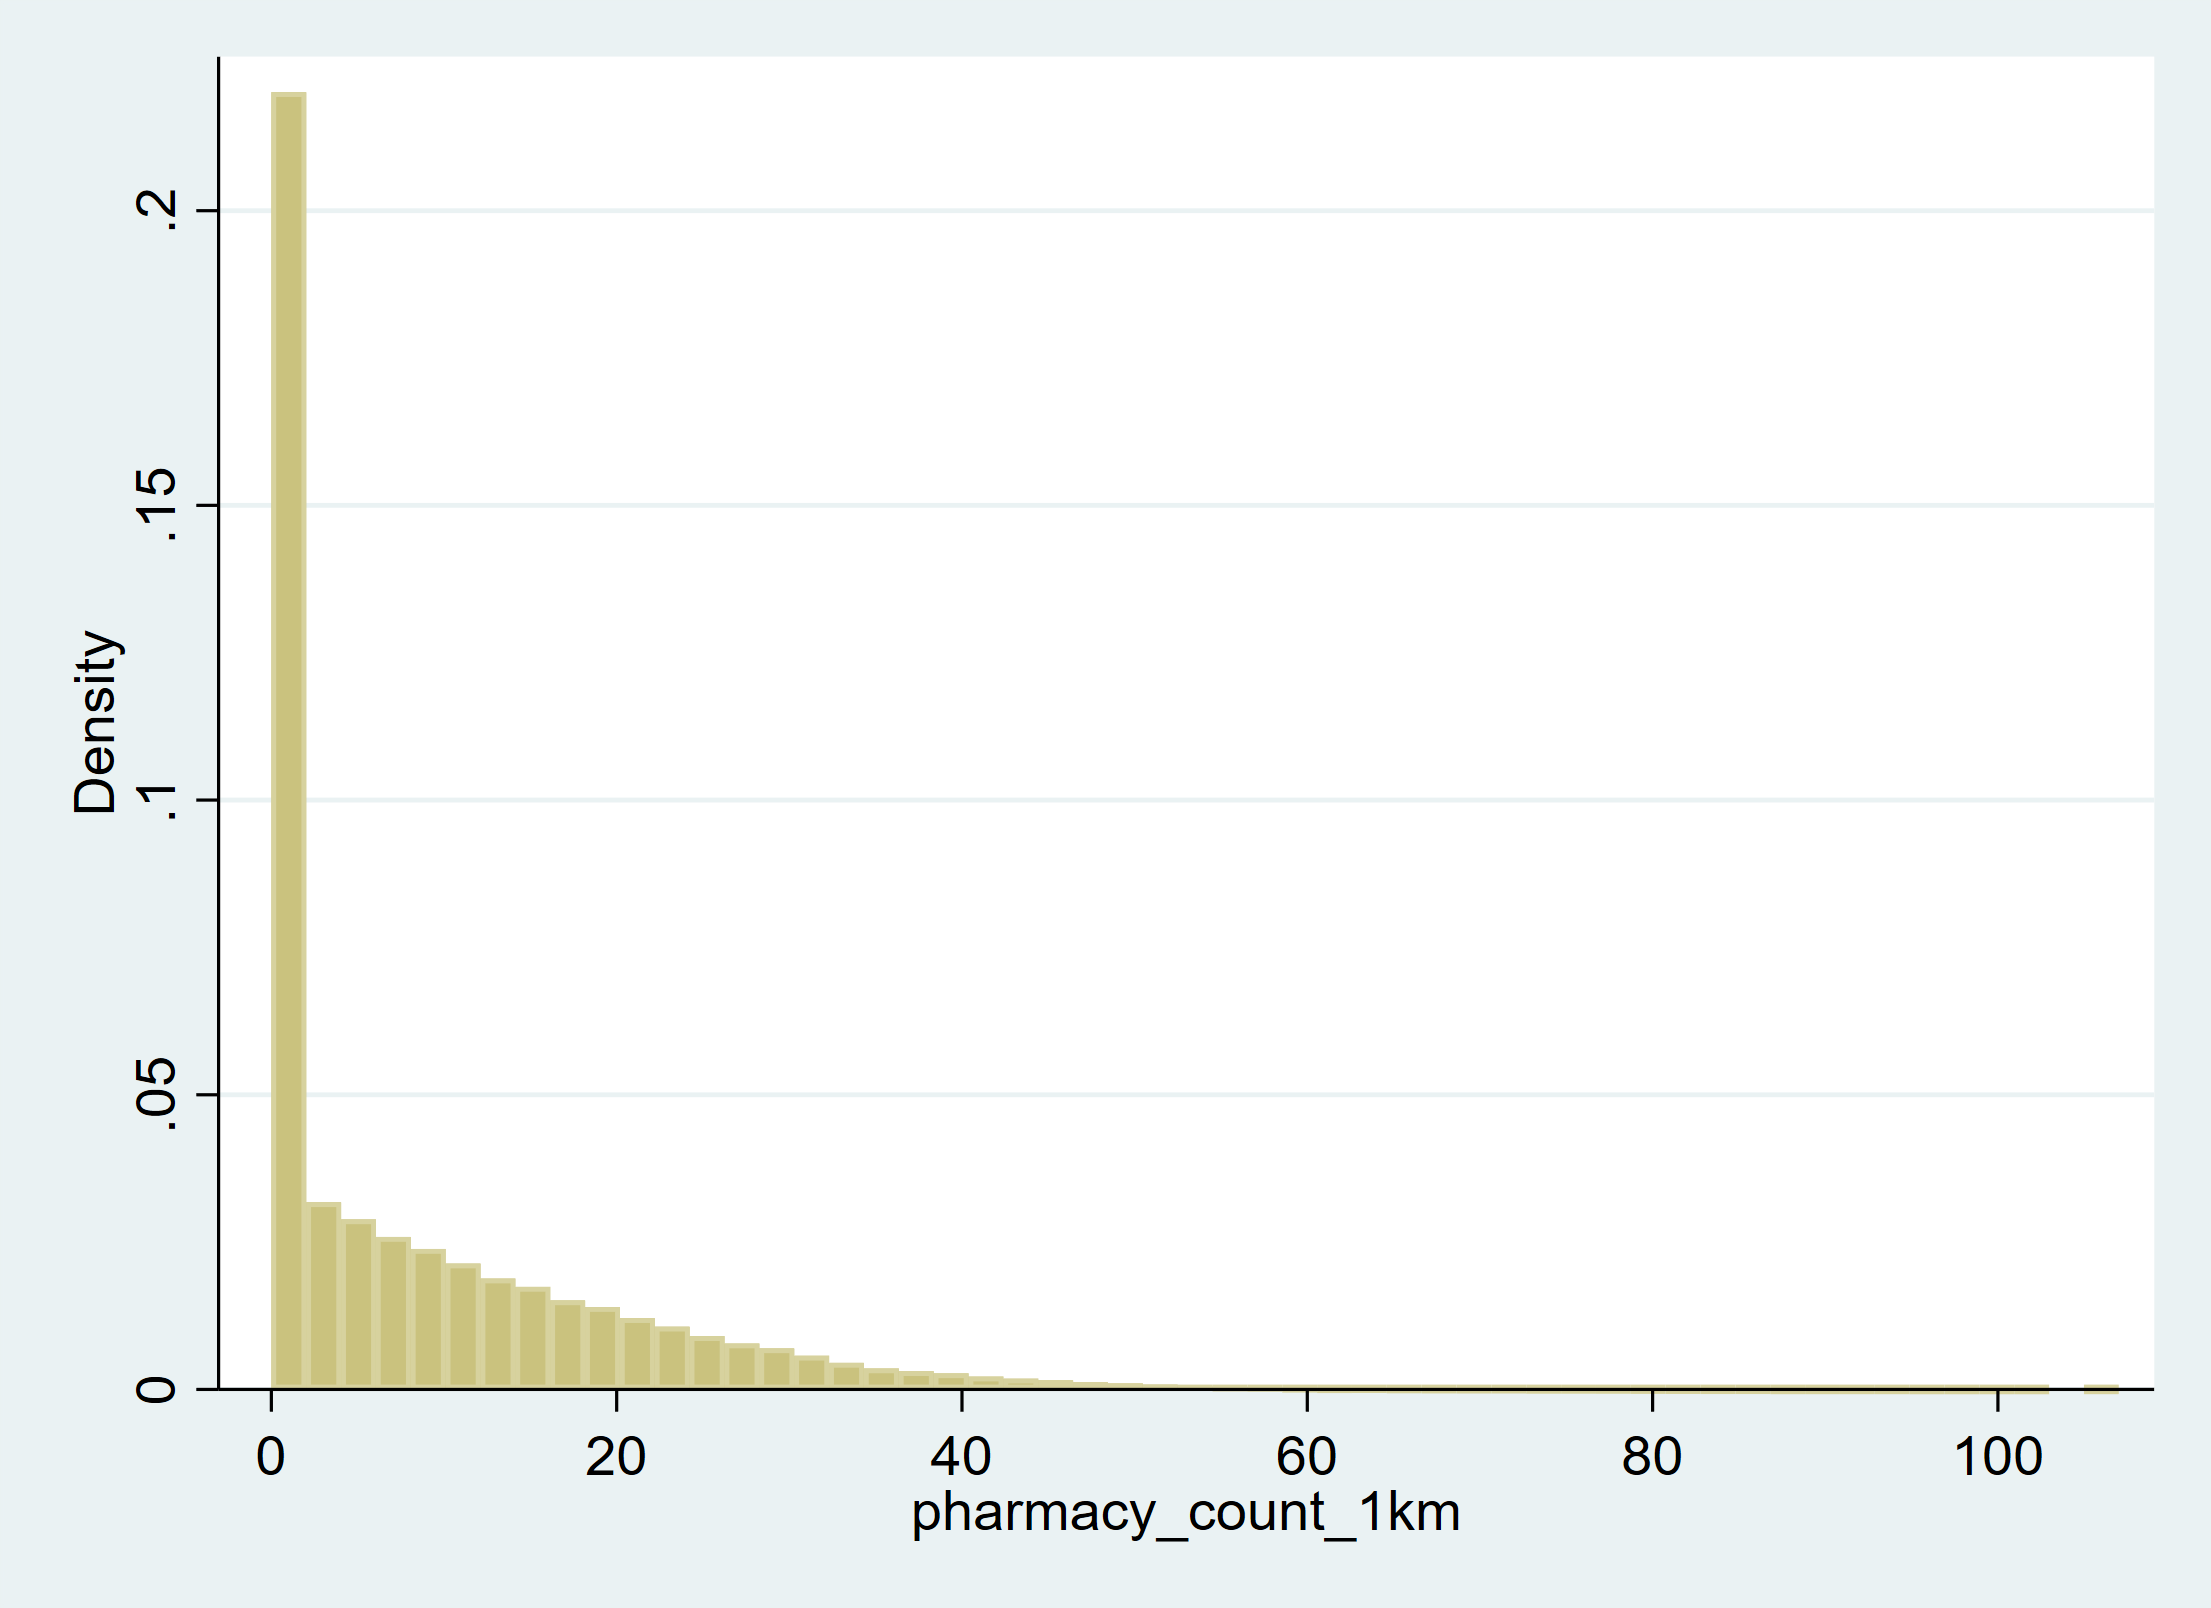
\includegraphics[width=\linewidth]{pharmacy_count_1km_density.png}

{\footnotesize (a) 1km}
\end{minipage}
\hfill
\begin{minipage}{0.32\textwidth}
\centering
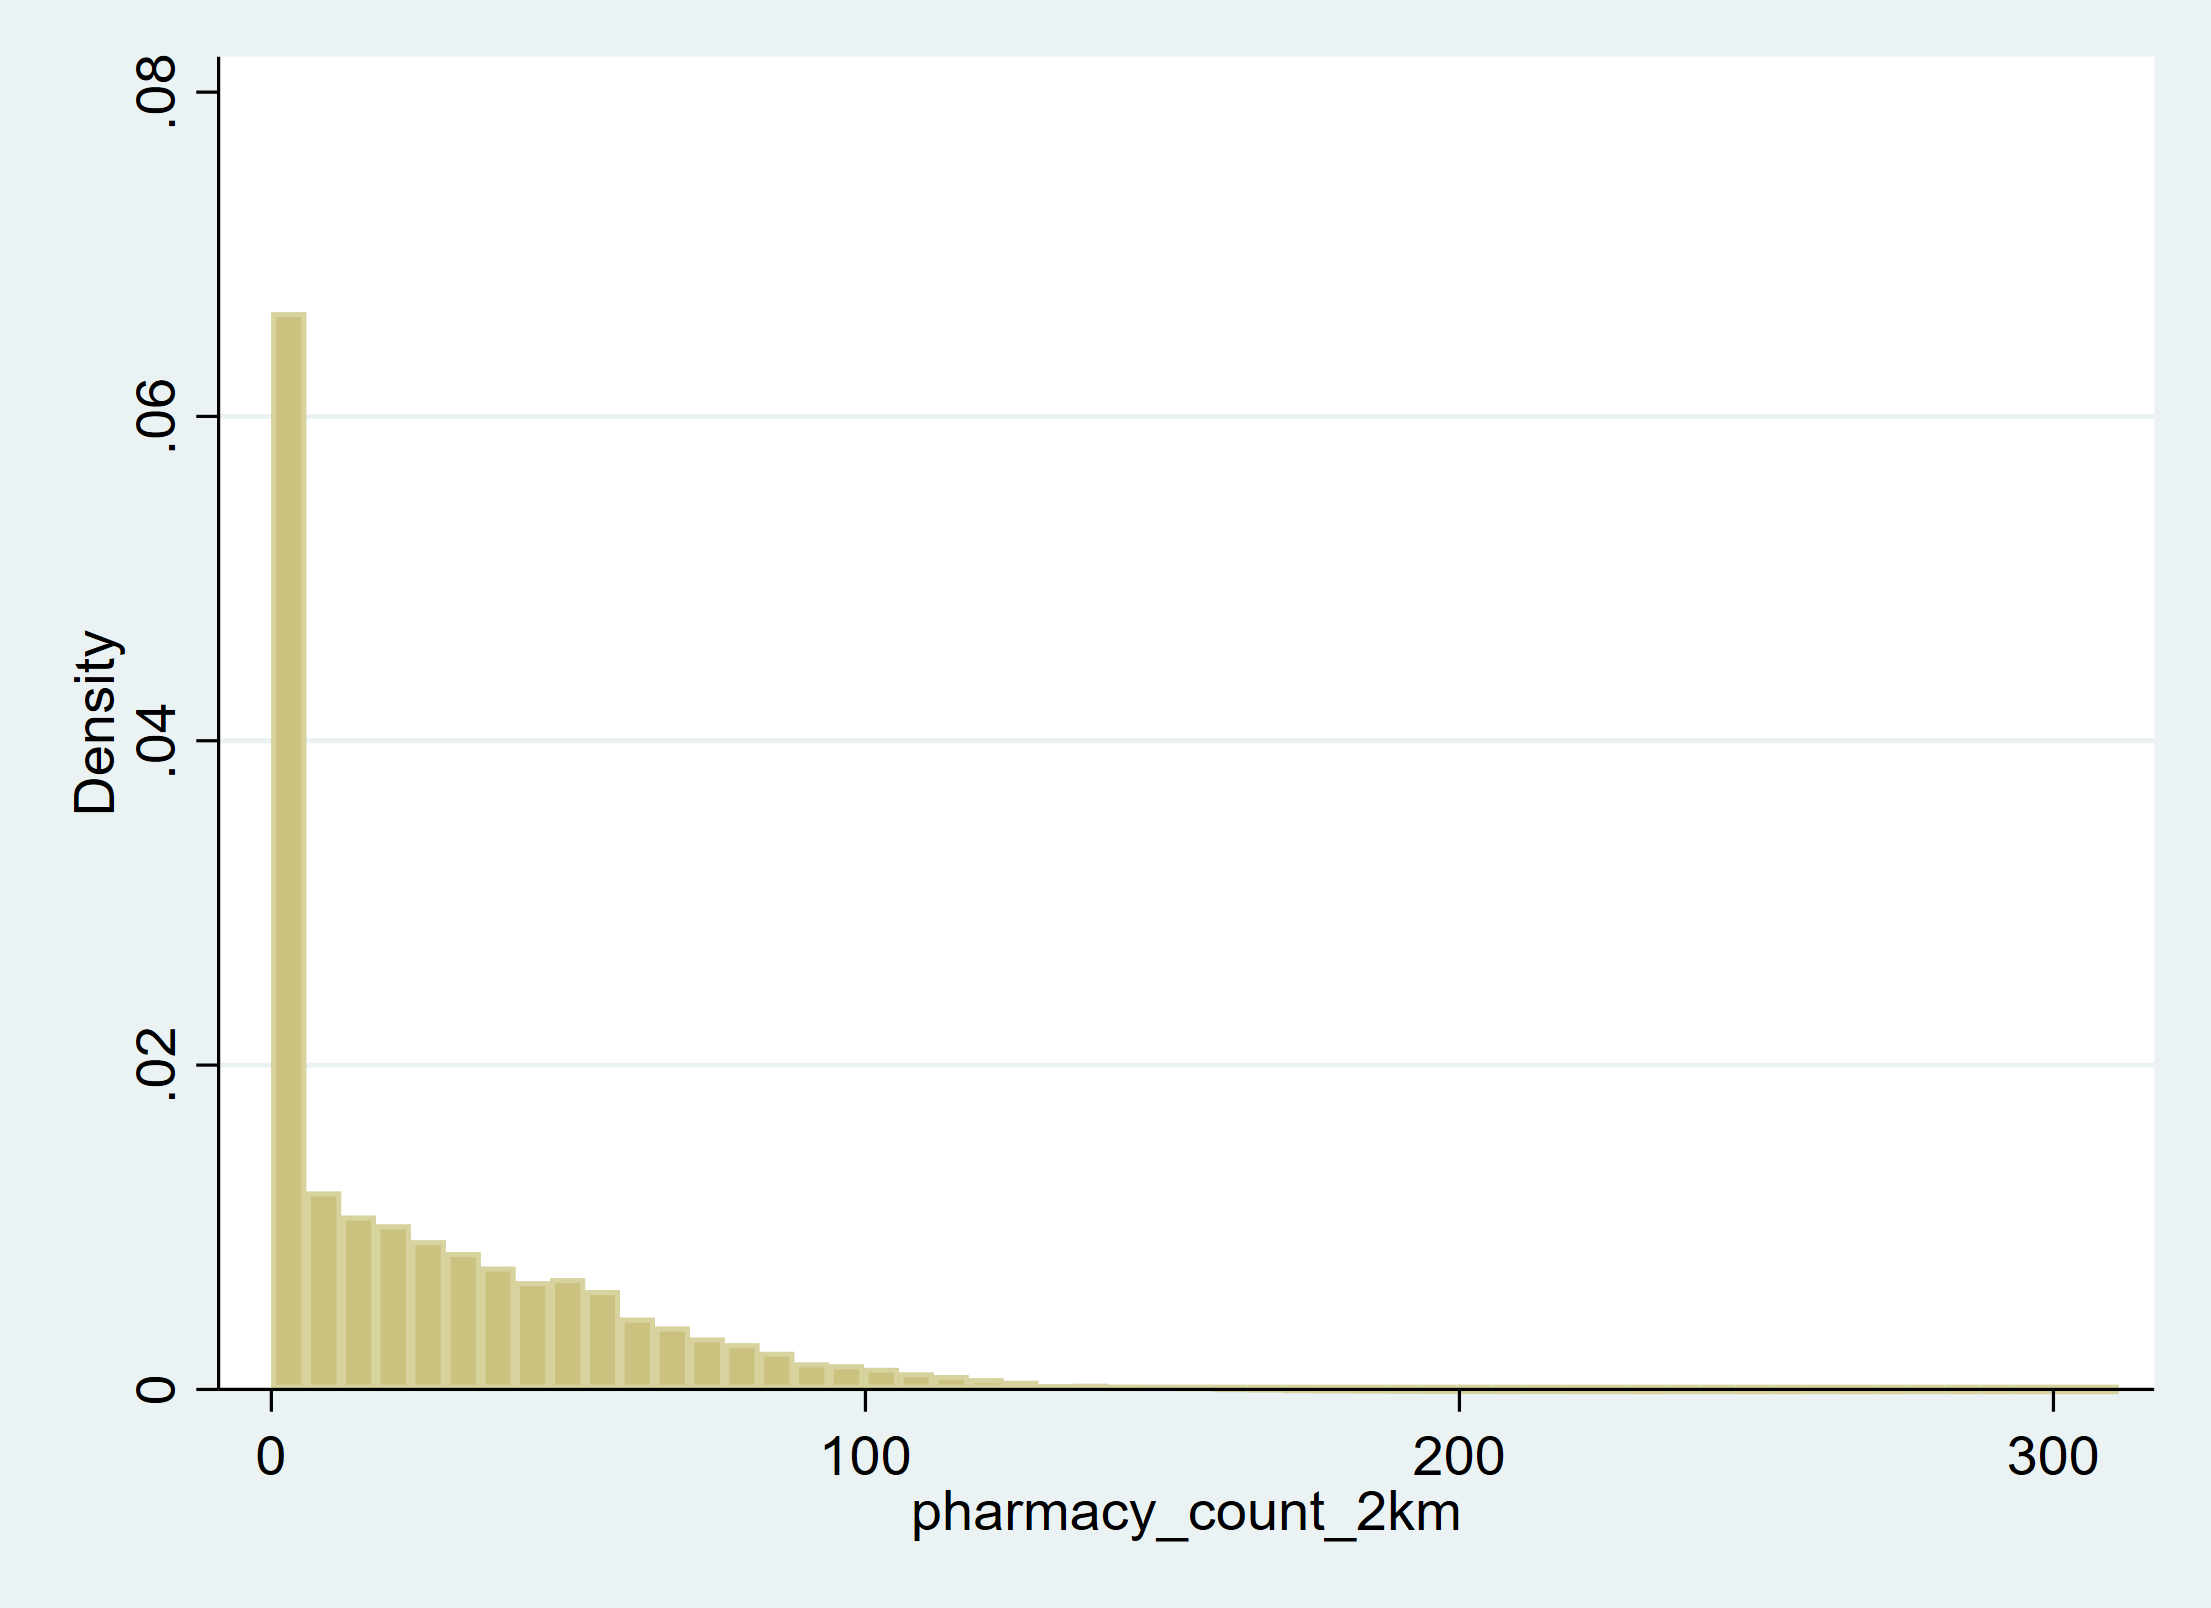
\includegraphics[width=\linewidth]{pharmacy_count_2km_density.png}

{\footnotesize (b) 2km}
\end{minipage}
\hfill
\begin{minipage}{0.32\textwidth}
\centering
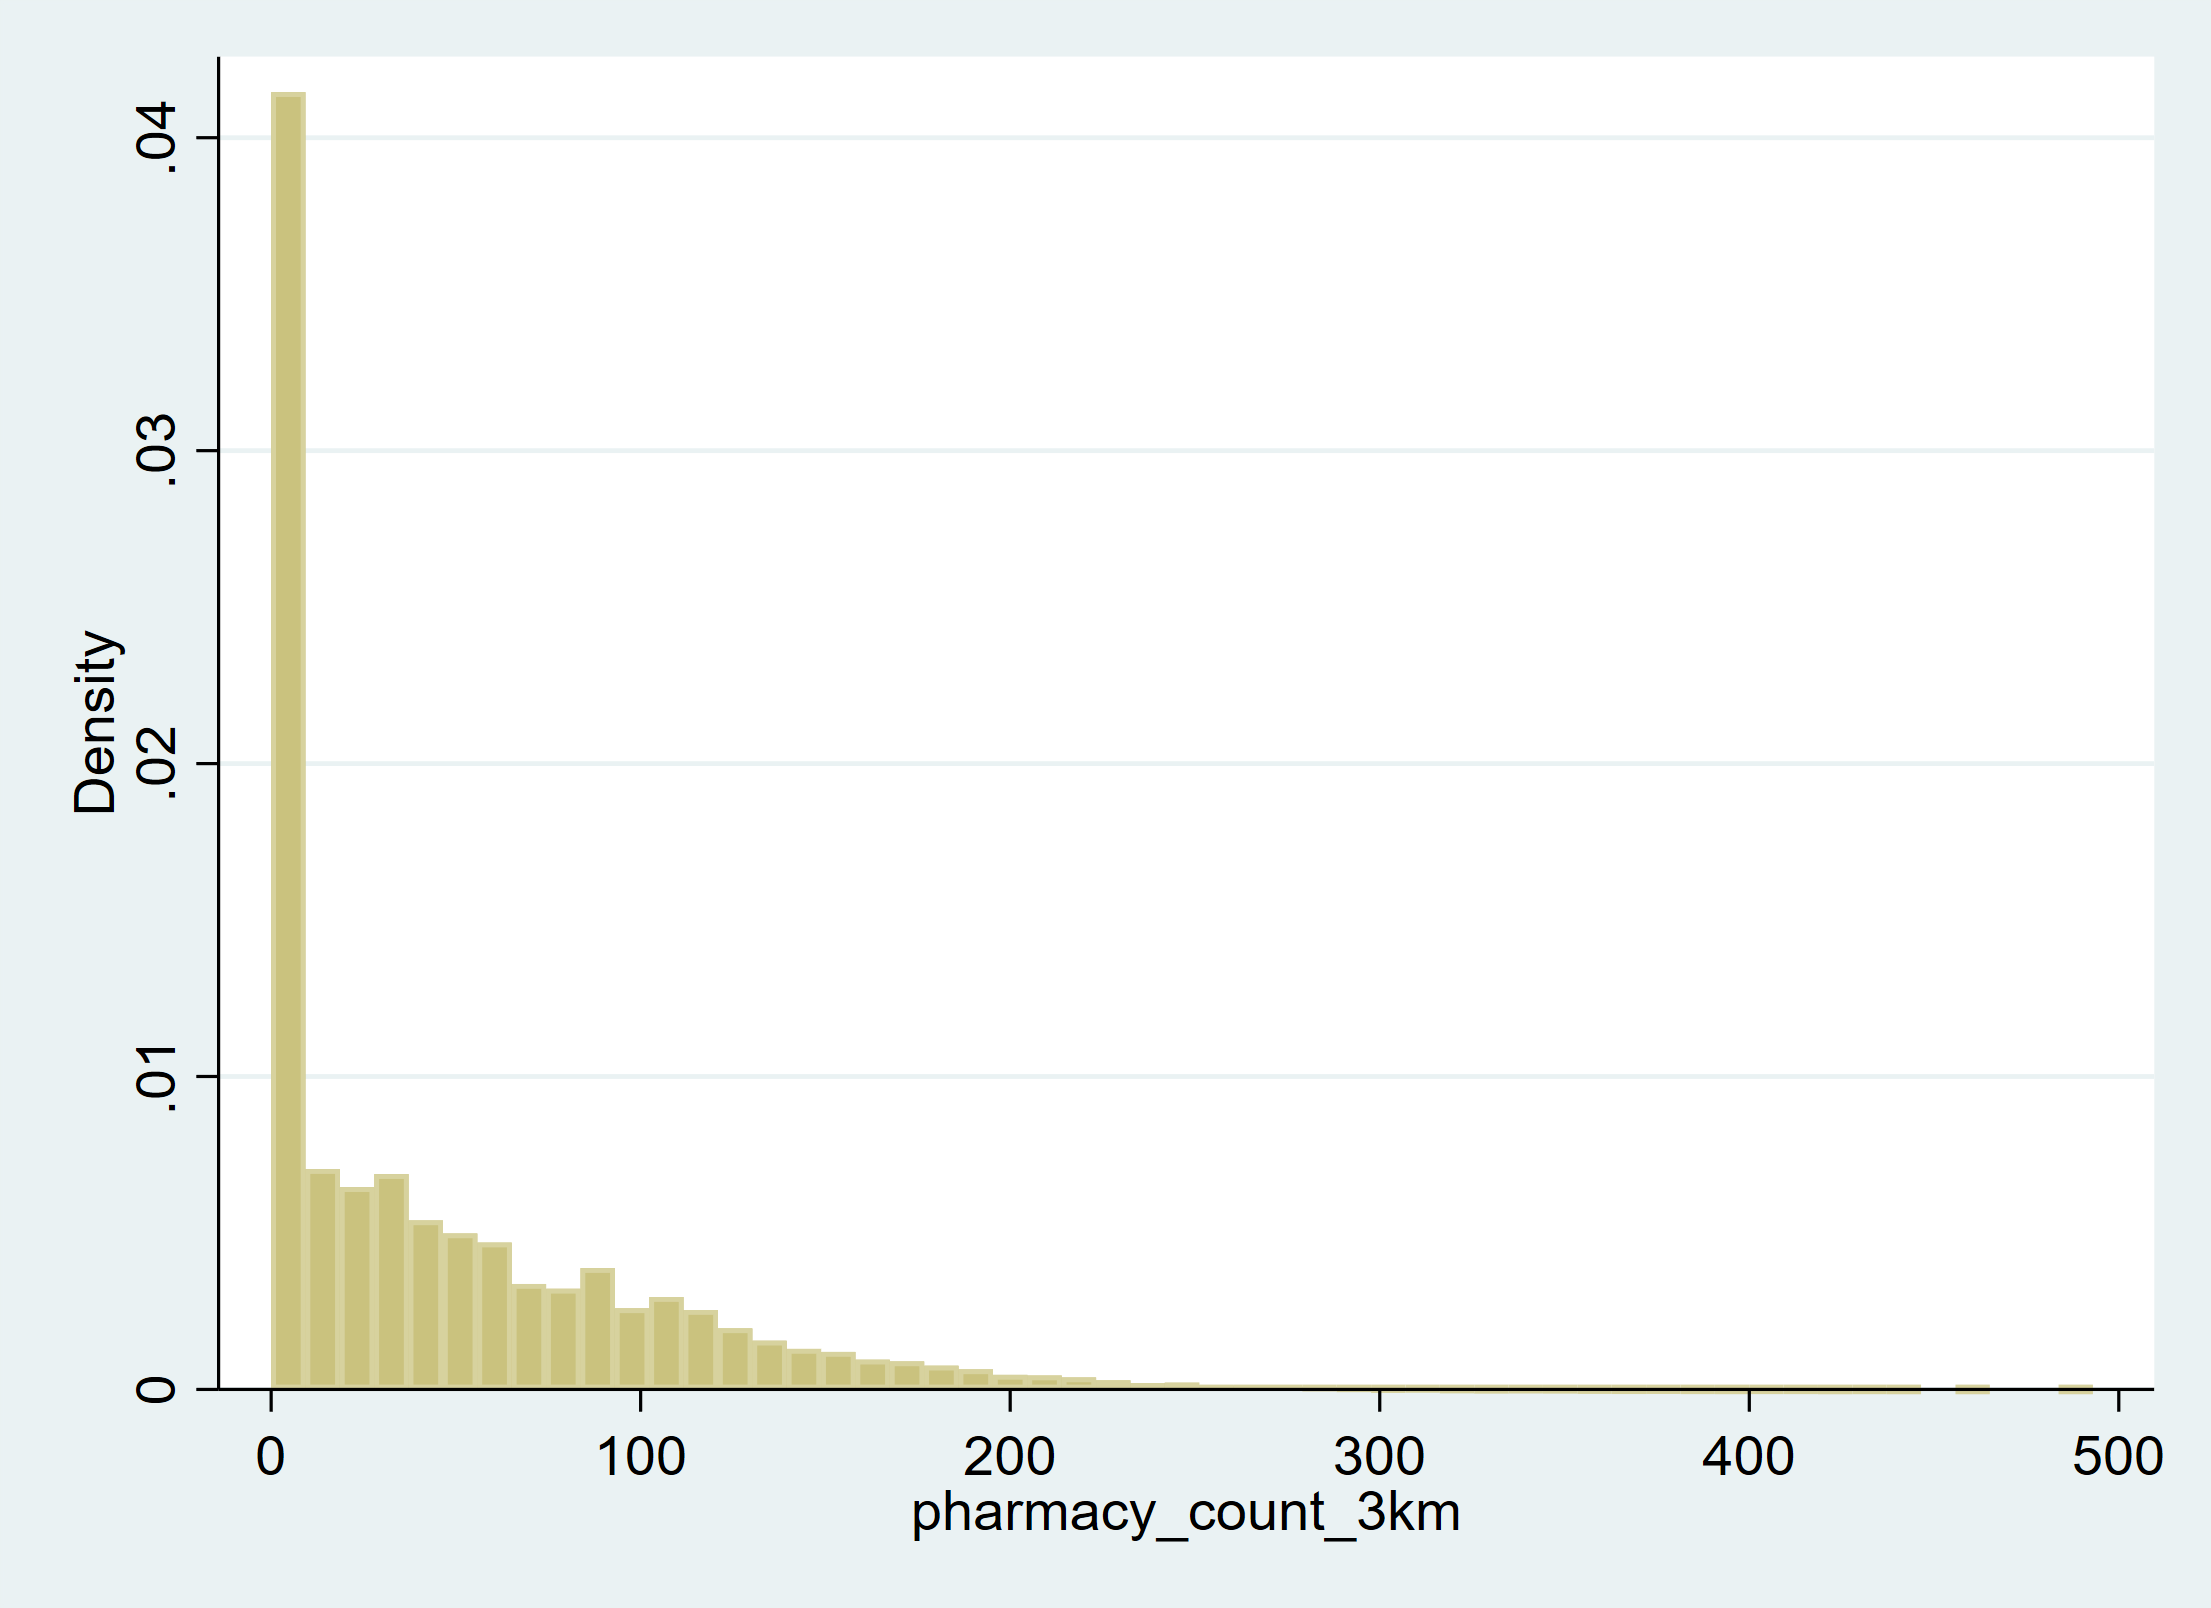
\includegraphics[width=\linewidth]{pharmacy_count_3km_density.png}

{\footnotesize (c) 3km}
\end{minipage}

\vspace{0.5em}
\footnotesize
Note: Distribution is highly right-skewed with mass at zero.

\end{frame}
% ================= Empirical Strategy =================
\begin{frame}{Empirical Strategy:TWFE}

\[
Y_{ict} = \beta_0+\beta_1 Reform_{ct}+\beta X_{ct} + \delta_i + \delta_t + \epsilon_{ict}
\]

\vspace{0.4cm}

\begin{itemize}
    \item $Y_{ict}$: Number of pharmacies around hospital $i$ in county $c$ at time $t$
    \item $Reform_{ct}$: Policy exposure at the county-year level
    \item $X_{ct}$: Control variables at the county-year level
    \item $\delta_i$: hospital fixed effects
    \item $\delta_t$: Year fixed effects
\end{itemize}

\vspace{0.4cm}

\centering
\textbf{\textbf{Traditional TWFE may be biased under staggered adoption}}

\end{frame}

\begin{frame}{Empirical Strategy: CS-DID}

\[
ATT(g,t) = \mathbb{E}[Y_t(1) - Y_t(0) \mid G = g]
\]

\vspace{0.4cm}

\begin{itemize}
    \item $g$: First year of reform (cohort)
    \item $t$: Year
    \item Compare treated units with not-yet-treated units
\end{itemize}

\vspace{0.4cm}

\begin{itemize}
    \item Allows for heterogeneous treatment effects
    \item Avoids bias from two-way fixed effects under staggered adoption
\end{itemize}

\vspace{0.4cm}

\centering
\textbf{Estimate dynamic and cohort-specific treatment effects}

\end{frame}


% ================= Baseline DID =================
\begin{frame}{Baseline DID Results:TWFE}

\textbf{OLS}

\begin{itemize}
    \item Outcome: Pharmacy entry around hospitals 
    \item Sample: score=10 | score=8
    \item Fixed effects: hospital and year
    \item Standard errors : clustered at  hospital level
\end{itemize}

\vspace{0.5em}
\centering
\footnotesize
\begin{tabular}{lccc}
\hline
\hline
 & (1) & (2) & (3) \\
 & pharmacy\textasciitilde 1km & pharmacy\textasciitilde 2km & pharmacy\textasciitilde 3km \\
\hline
did & -0.433*** & -0.942*** & -1.101* \\
 & (0.103) & (0.263) & (0.449) \\
\hline
N & 193010 & 193010 & 193010 \\
R-sq & 0.884 & 0.895 & 0.903 \\
\hline
\hline
\end{tabular}
\end{frame}


% ========== OLS第二个回归结果（county level)==========
\begin{frame}{Baseline DID Results:TWFE}

\textbf{OLS}

\begin{itemize}
    \item Outcome: Pharmacy entry around hospitals 
    \item Sample: score=10 | score=8
    \item Fixed effects: Hospital and year
    \item Standard errors : clustered at  county level  
\end{itemize}

\vspace{0.5em}
\centering
\footnotesize
\begin{tabular}{lccc}
\hline
\hline
 & (1) & (2) & (3) \\
 & pharmacy\textasciitilde 1km & pharmacy\textasciitilde 2km & pharmacy\textasciitilde 3km \\
\hline
did & -0.433** & -0.947* & -1.113 \\
 & (0.161) & (0.441) & (0.776) \\
\hline
N & 192868 & 192868 & 192868 \\
R-sq & 0.884 & 0.895 & 0.903 \\
\hline
\hline
\end{tabular}

\end{frame}

% ========== CS-DID回归结果（id level)==========
\begin{frame}{Baseline DID Results: CS-DID}

\textbf{Callaway and Sant'Anna(2021)}

\begin{itemize}
    \item Outcome model  : least squares
    \item Control: never treated
    \item Treatment model: inverse probability
    \item Standard errors : clustered at  hospital level
\end{itemize}

\vspace{0.5em}
\centering
\footnotesize
\begin{tabular}{lccc}
\toprule
 & (1) & (2) & (3) \\
 & pharmacy\textasciitilde 1km & pharmacy\textasciitilde 2km & pharmacy\textasciitilde 3km \\
\midrule
ATT & -0.0736  &  -.320526      &    -.5840457      \\
    & (0.0985) &   (.2412168)       &  (.4028106)      \\
\midrule
N   & 124137   & 124137   & 124137  \\
\bottomrule
\end{tabular}


\end{frame}

% ========== CS-DID回归结果（county level)==========
\begin{frame}{Baseline DID Results: CS-DID}

\textbf{Callaway and Sant'Anna(2021)}

\begin{itemize}
    \item Outcome model  : least squares
    \item Control: never treated
    \item Treatment model: inverse probability
    \item Standard errors : clustered at  county level
\end{itemize}

\vspace{0.5em}
\centering
\footnotesize
\begin{tabular}{lccc}
\toprule
 & (1) & (2) & (3) \\
 & pharmacy\textasciitilde 1km & pharmacy\textasciitilde 2km & pharmacy\textasciitilde 3km \\
\midrule
ATT &  -.0735517  &   -.320526       &    -.5840457      \\
    & (.0985356) &   ( .2412168)       &  (.4028106 )      \\
\midrule
N   &  124137   & 124137   & 124137  \\
\bottomrule
\end{tabular}


\end{frame}
% ========== PPML回归结果（id level)==========

\begin{frame}{Baseline DID Results: PPML}

\textbf{PPML}

\begin{itemize}
    \item Outcome: Pharmacy entry around hospitals
    \item Fixed effects: hospital and year
    \item Sample: score=10 | score=8
    \item Standard errors : clustered at hospital level
\end{itemize}

\vspace{0.5em}
\centering
\footnotesize
\begin{tabular}{lccc}
\hline
\hline
 & (1) & (2) & (3) \\
 & pharmacy\textasciitilde 1km & pharmacy\textasciitilde 2km & pharmacy\textasciitilde 3km \\
\hline
did & 0.042*** & 0.049*** & 0.058*** \\
 & (0.009) & (0.009) & (0.009) \\
\hline
N & 173450 & 181287 & 183995 \\
\hline
\hline
\end{tabular}

\end{frame}

% ========== PPML回归结果（county_id level)==========

\begin{frame}{Baseline DID Results: PPML}

\textbf{PPML}

\begin{itemize}
    \item Outcome: Pharmacy entry around hospitals
    \item Fixed effects: hospital and year
    \item Sample: score=10 | score=8
    \item Standard errors : clustered at county level
\end{itemize}

\vspace{0.5em}
\centering
\footnotesize
\begin{tabular}{lccc}
\hline
\hline
 & (1) & (2) & (3) \\
 & pharmacy\textasciitilde 1km & pharmacy\textasciitilde 2km & pharmacy\textasciitilde 3km \\
\hline
did & 0.043*** & 0.050*** & 0.058*** \\
 & (0.016) & (0.015) & (0.016) \\
\hline
N &  173319  & 181145 &  183853  \\
\hline
\hline
\end{tabular}

\end{frame}




% ========== Event Study:PPML==========
\begin{frame}{Event Study:PPML}


\begin{itemize}
    \item Outcome: Pharmacy entry around hospitals (within 1km)
    \item Fixed effects: hospital and year
    \item Standard errors : clustered at  county level
\end{itemize}

\vspace{0.5em}
\begin{center}
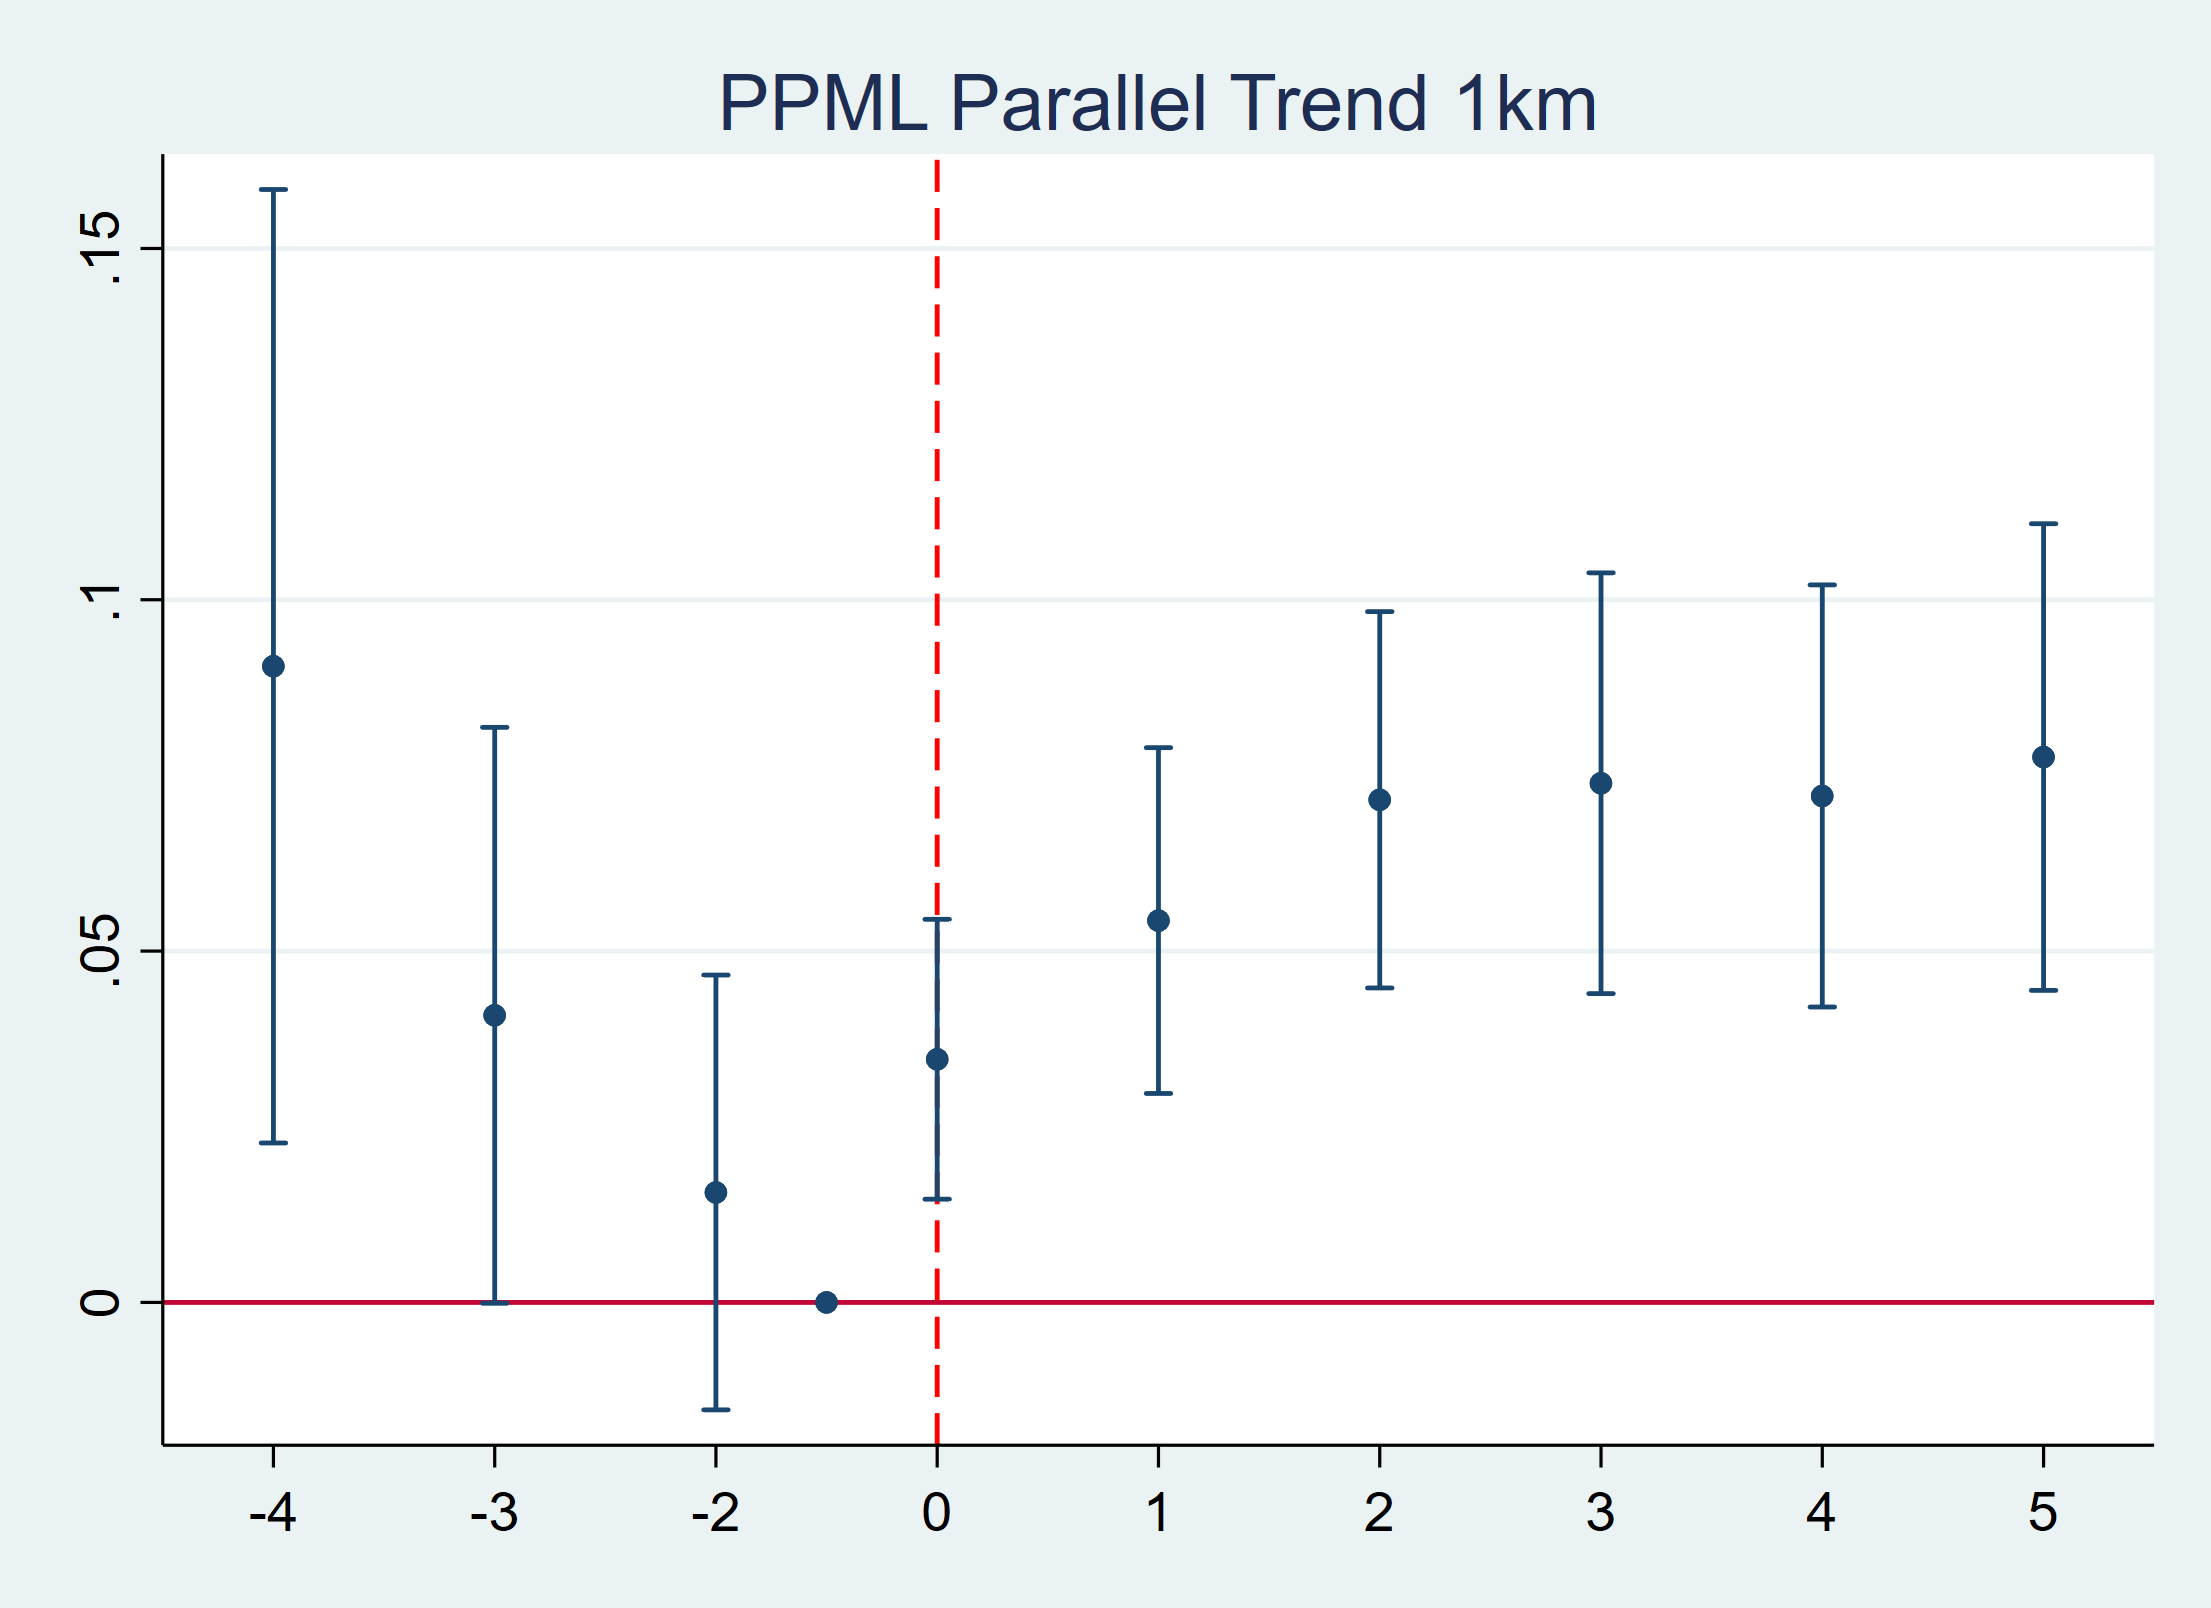
\includegraphics[width=0.8\textwidth]{parallel_ppml_1km.png}
\end{center}

\end{frame}

\begin{frame}{Event Study:PPML}



\begin{itemize}
    \item Outcome: Pharmacy entry around hospitals (within 2km)
    \item Fixed effects: hospital and year
    \item Standard errors : clustered at  county level
\end{itemize}

\vspace{0.5em}
\begin{center}
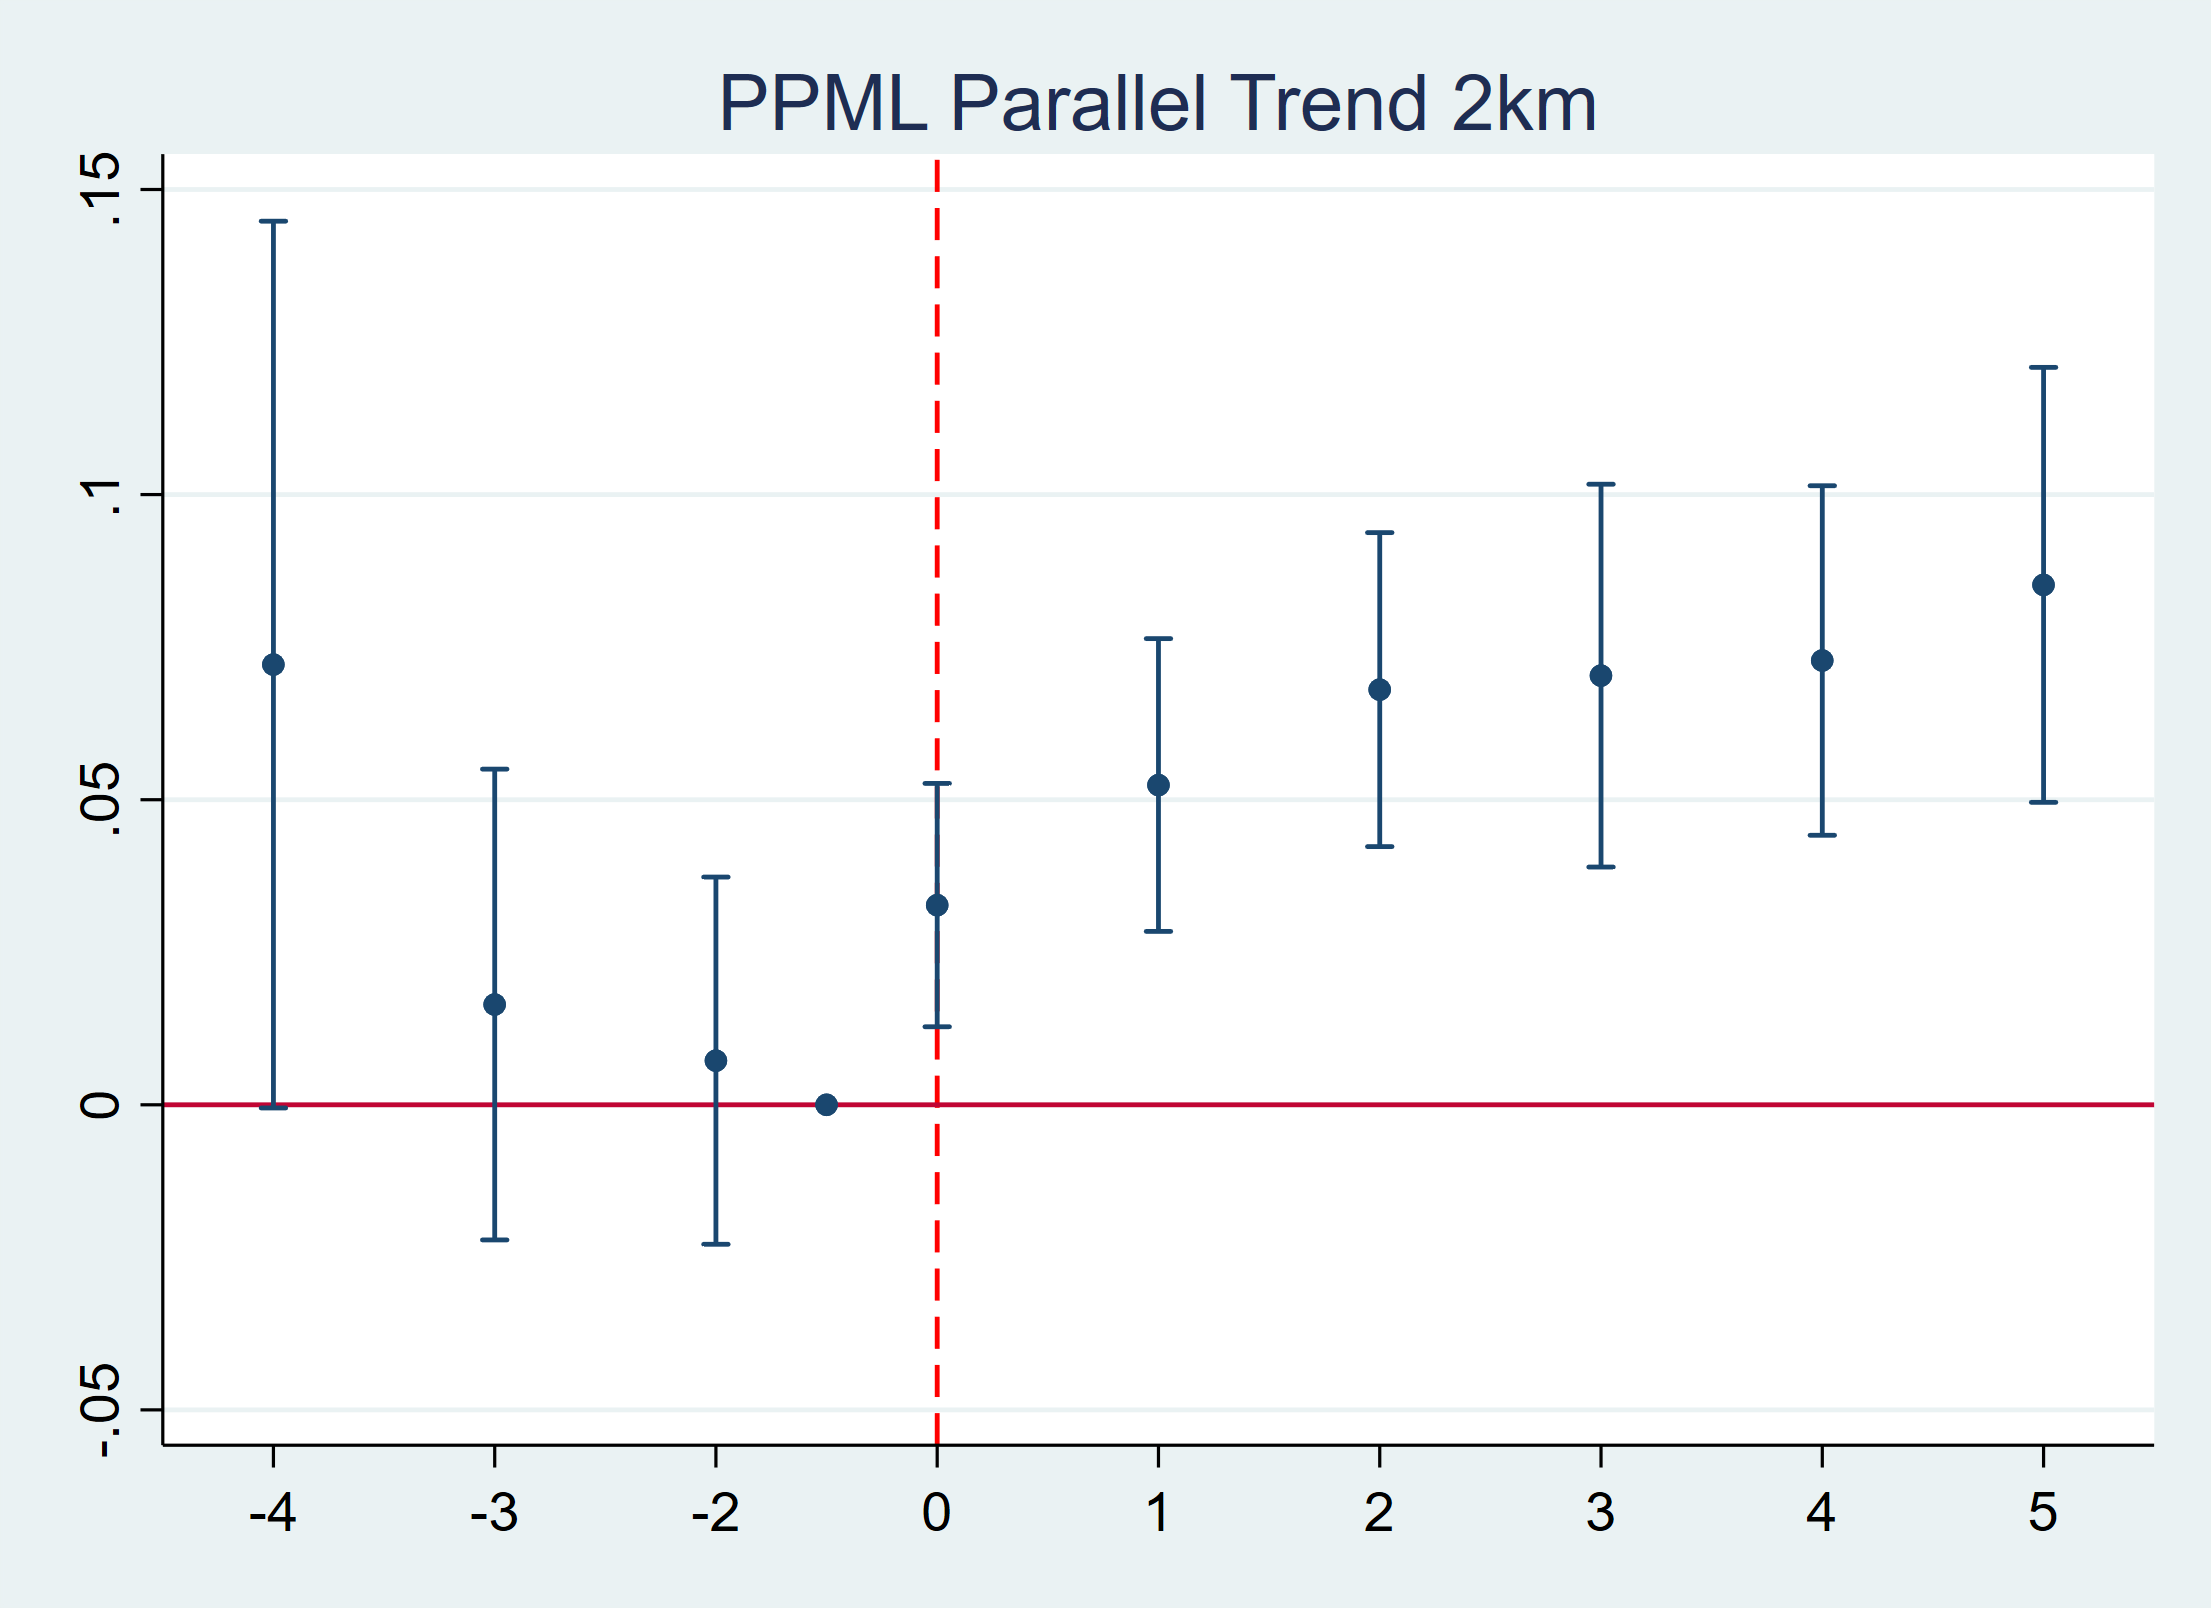
\includegraphics[width=0.8\textwidth]{parallel_ppml_2km.png}
\end{center}

\end{frame}


\begin{frame}{Event Study:PPML}

\begin{itemize}
    \item Outcome: Pharmacy entry around hospitals (within 3km)
    \item Fixed effects: hospital and year
    \item Standard errors : clustered at  county level
\end{itemize}

\vspace{0.5em}
\begin{center}
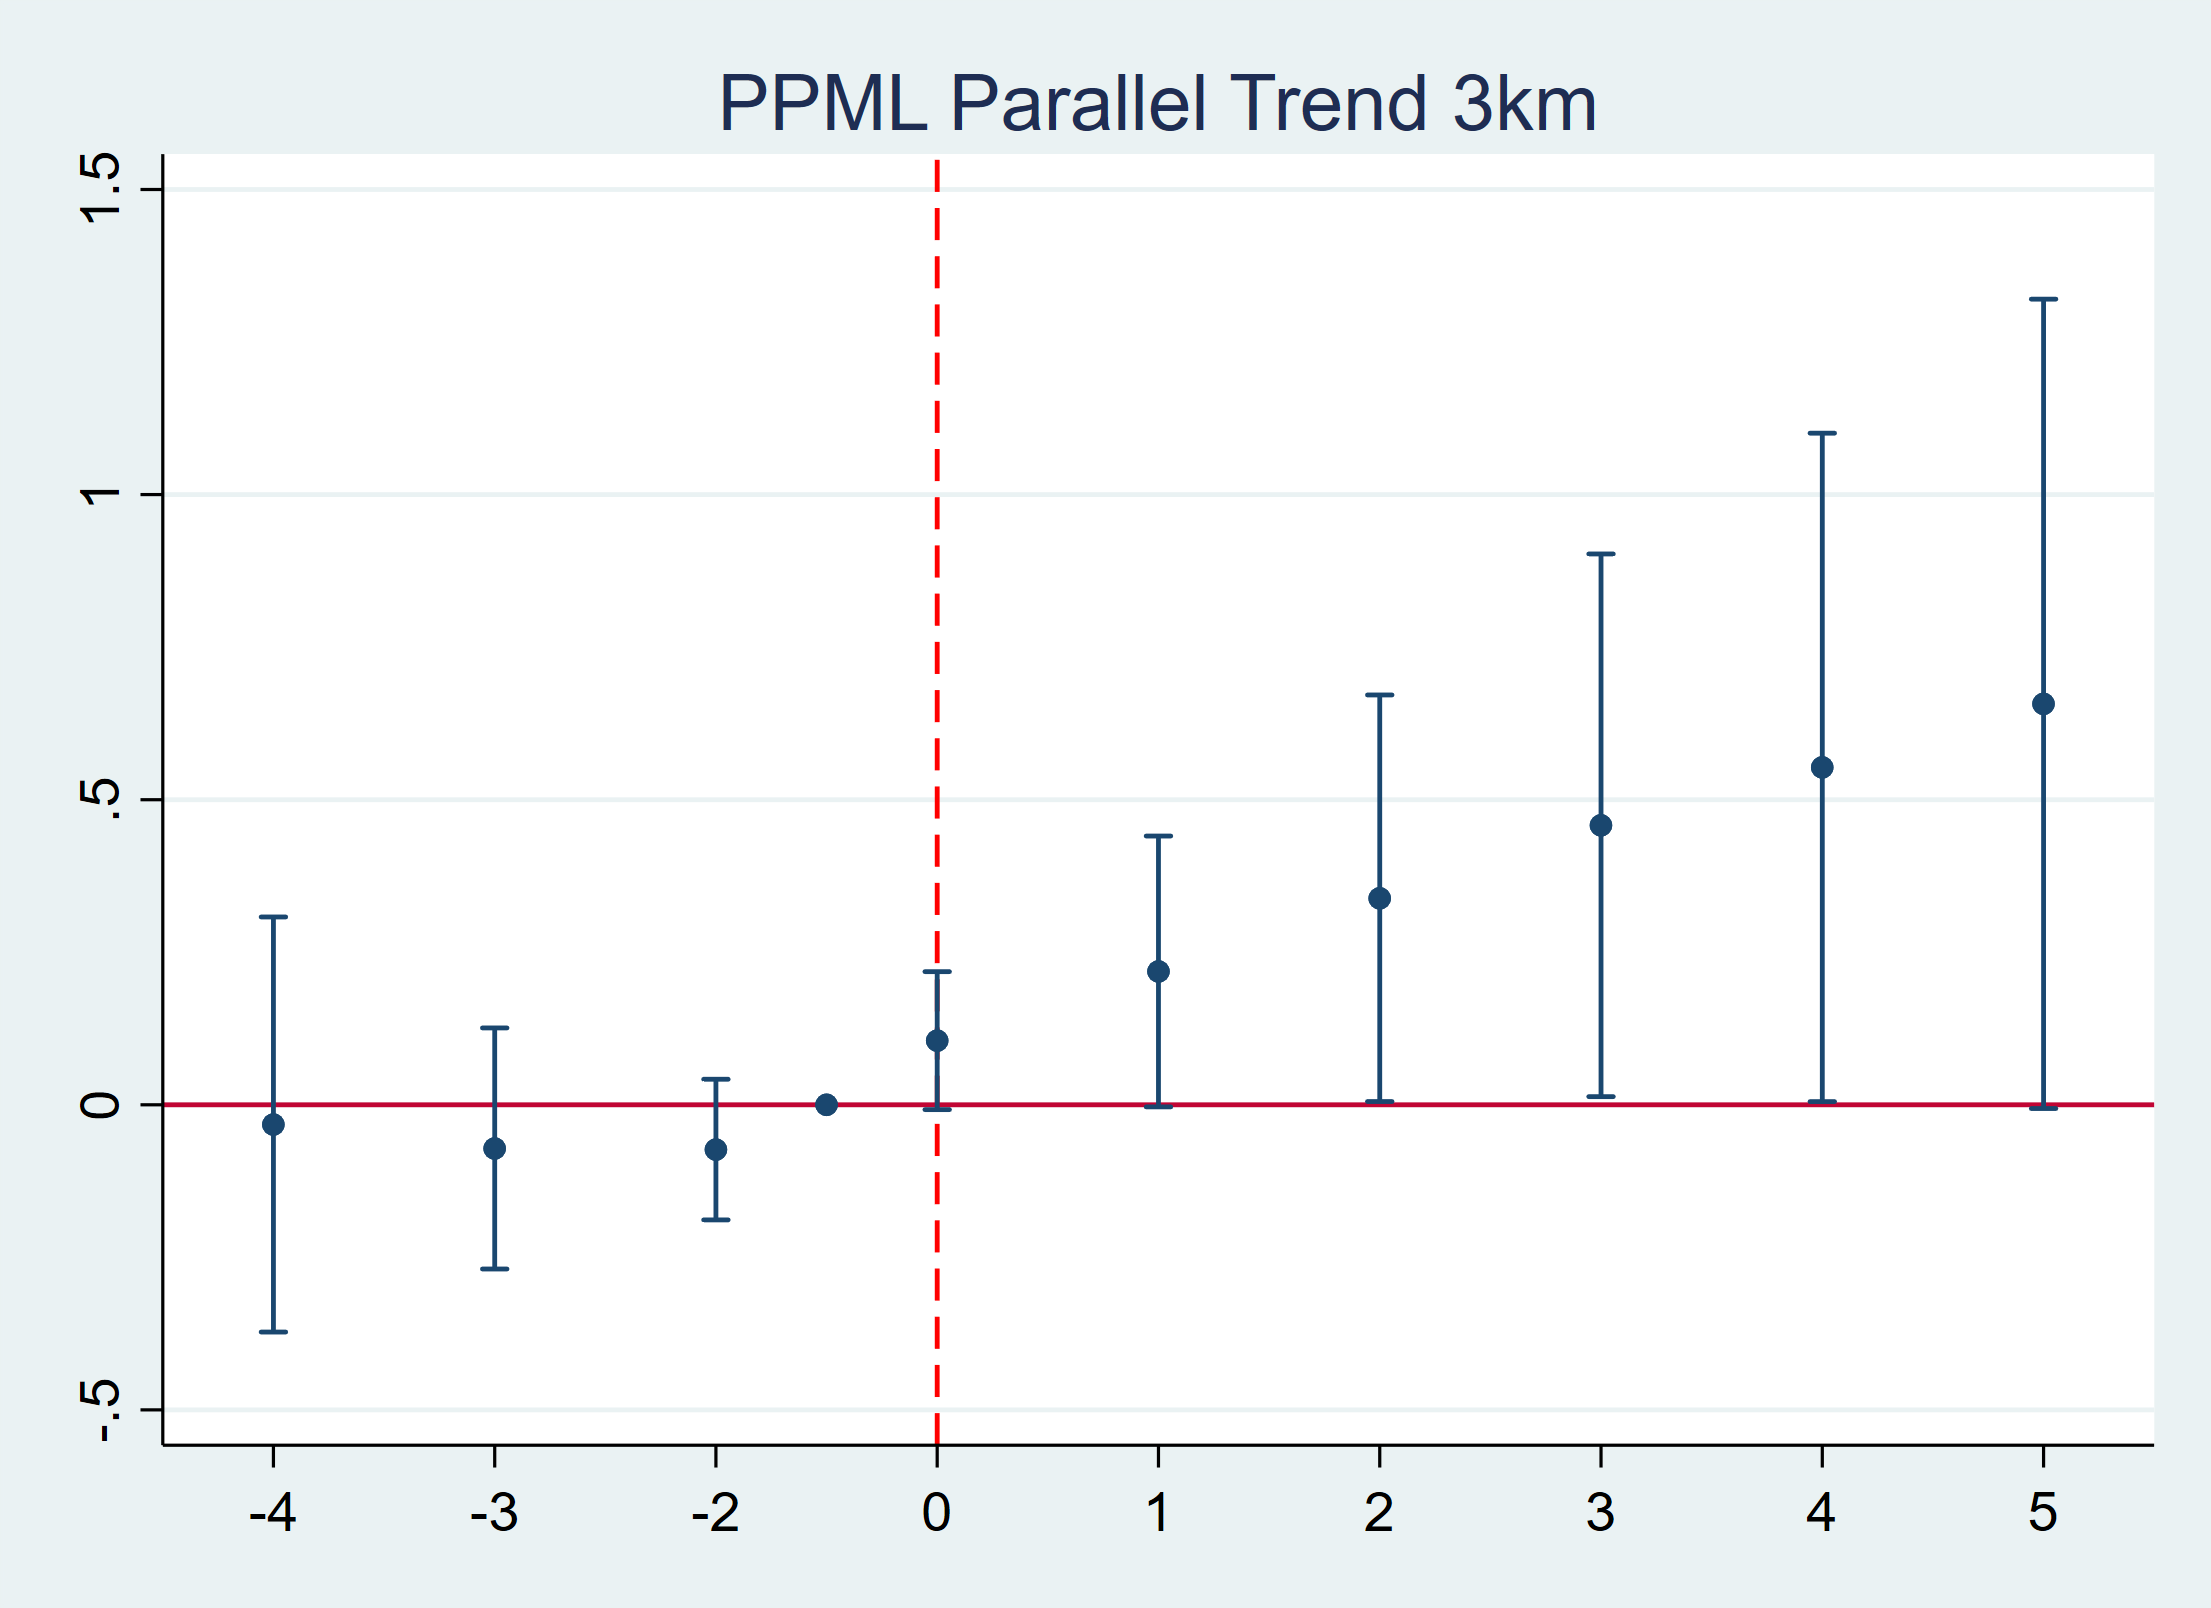
\includegraphics[width=0.8\textwidth]{parallel_ppml_3km.png}
\end{center}

\end{frame}

% ========== Event Study:TWFE==========
\begin{frame}{Event Study:TWFE}

\begin{itemize}
    \item Outcome: Pharmacy entry around hospitals (within 1km)
    \item Fixed effects: hospital and year
    \item Standard errors : clustered at  county level
\end{itemize}

\vspace{0.5em}
\begin{center}
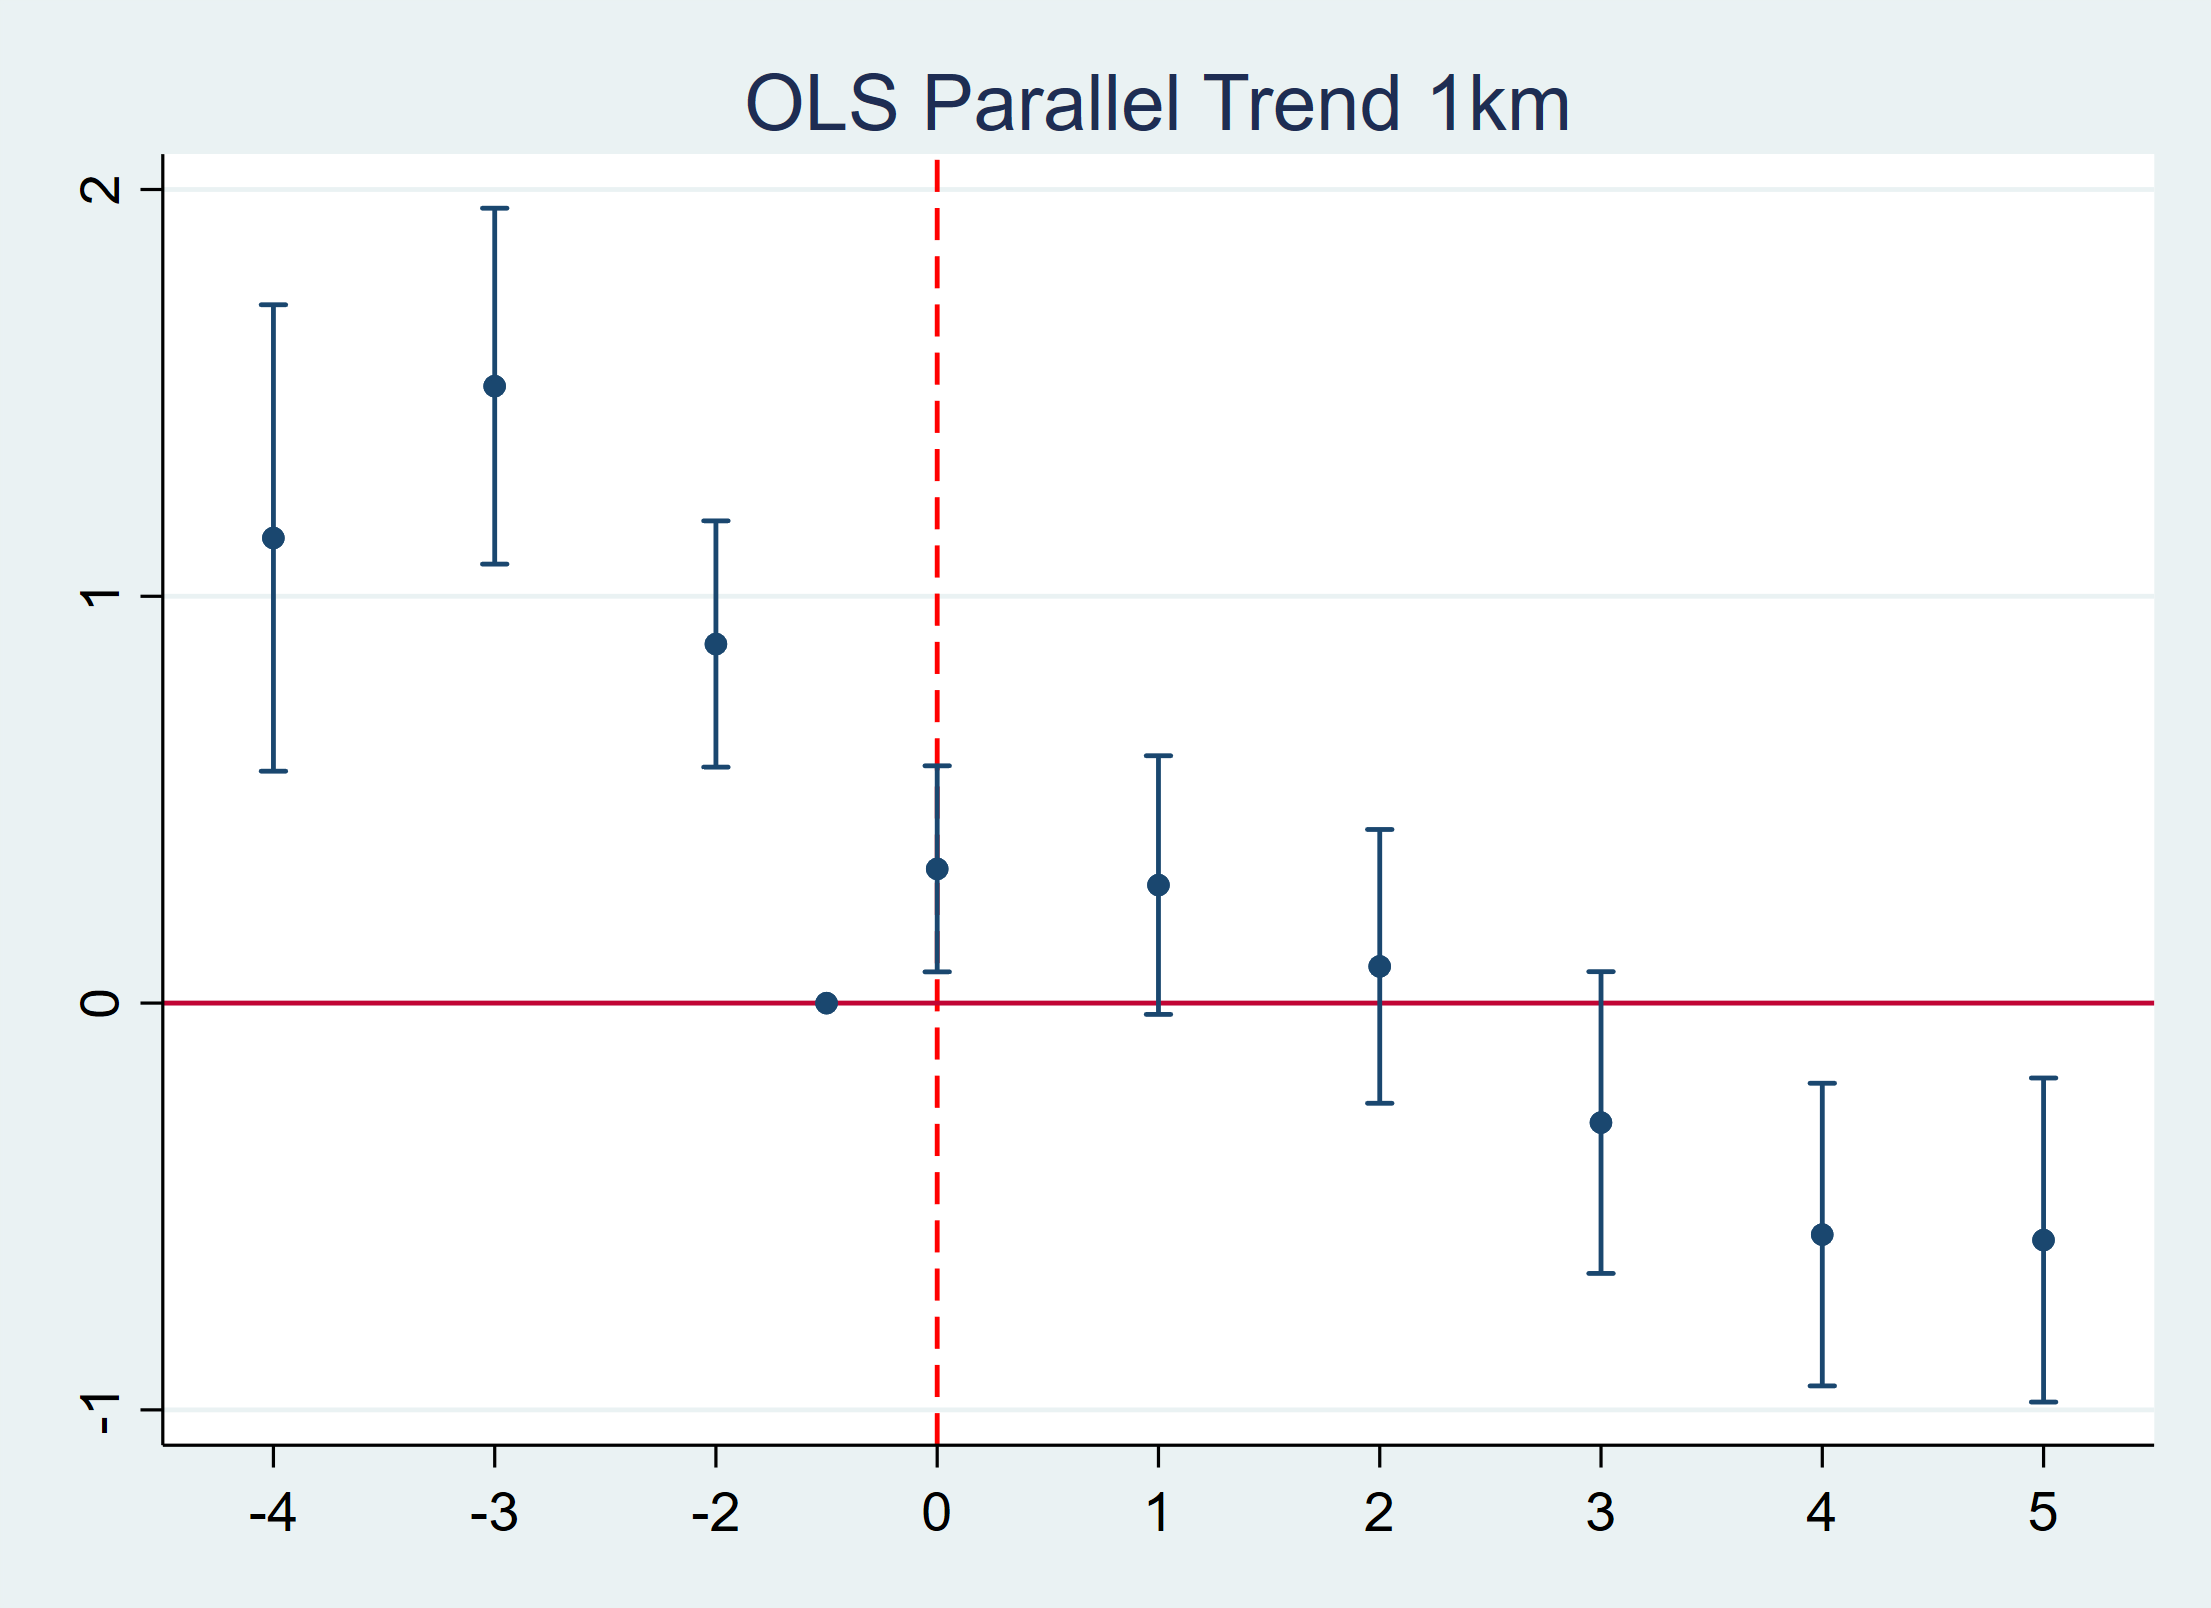
\includegraphics[width=0.8\textwidth]{parallel_ols_1km.png}
\end{center}

\end{frame}

\begin{frame}{Event Study:TWFE}

\begin{itemize}
    \item Outcome: Pharmacy entry around hospitals (within 2km)
    \item Fixed effects: hospital and year
    \item Standard errors : clustered at  county level
\end{itemize}

\vspace{0.5em}
\begin{center}
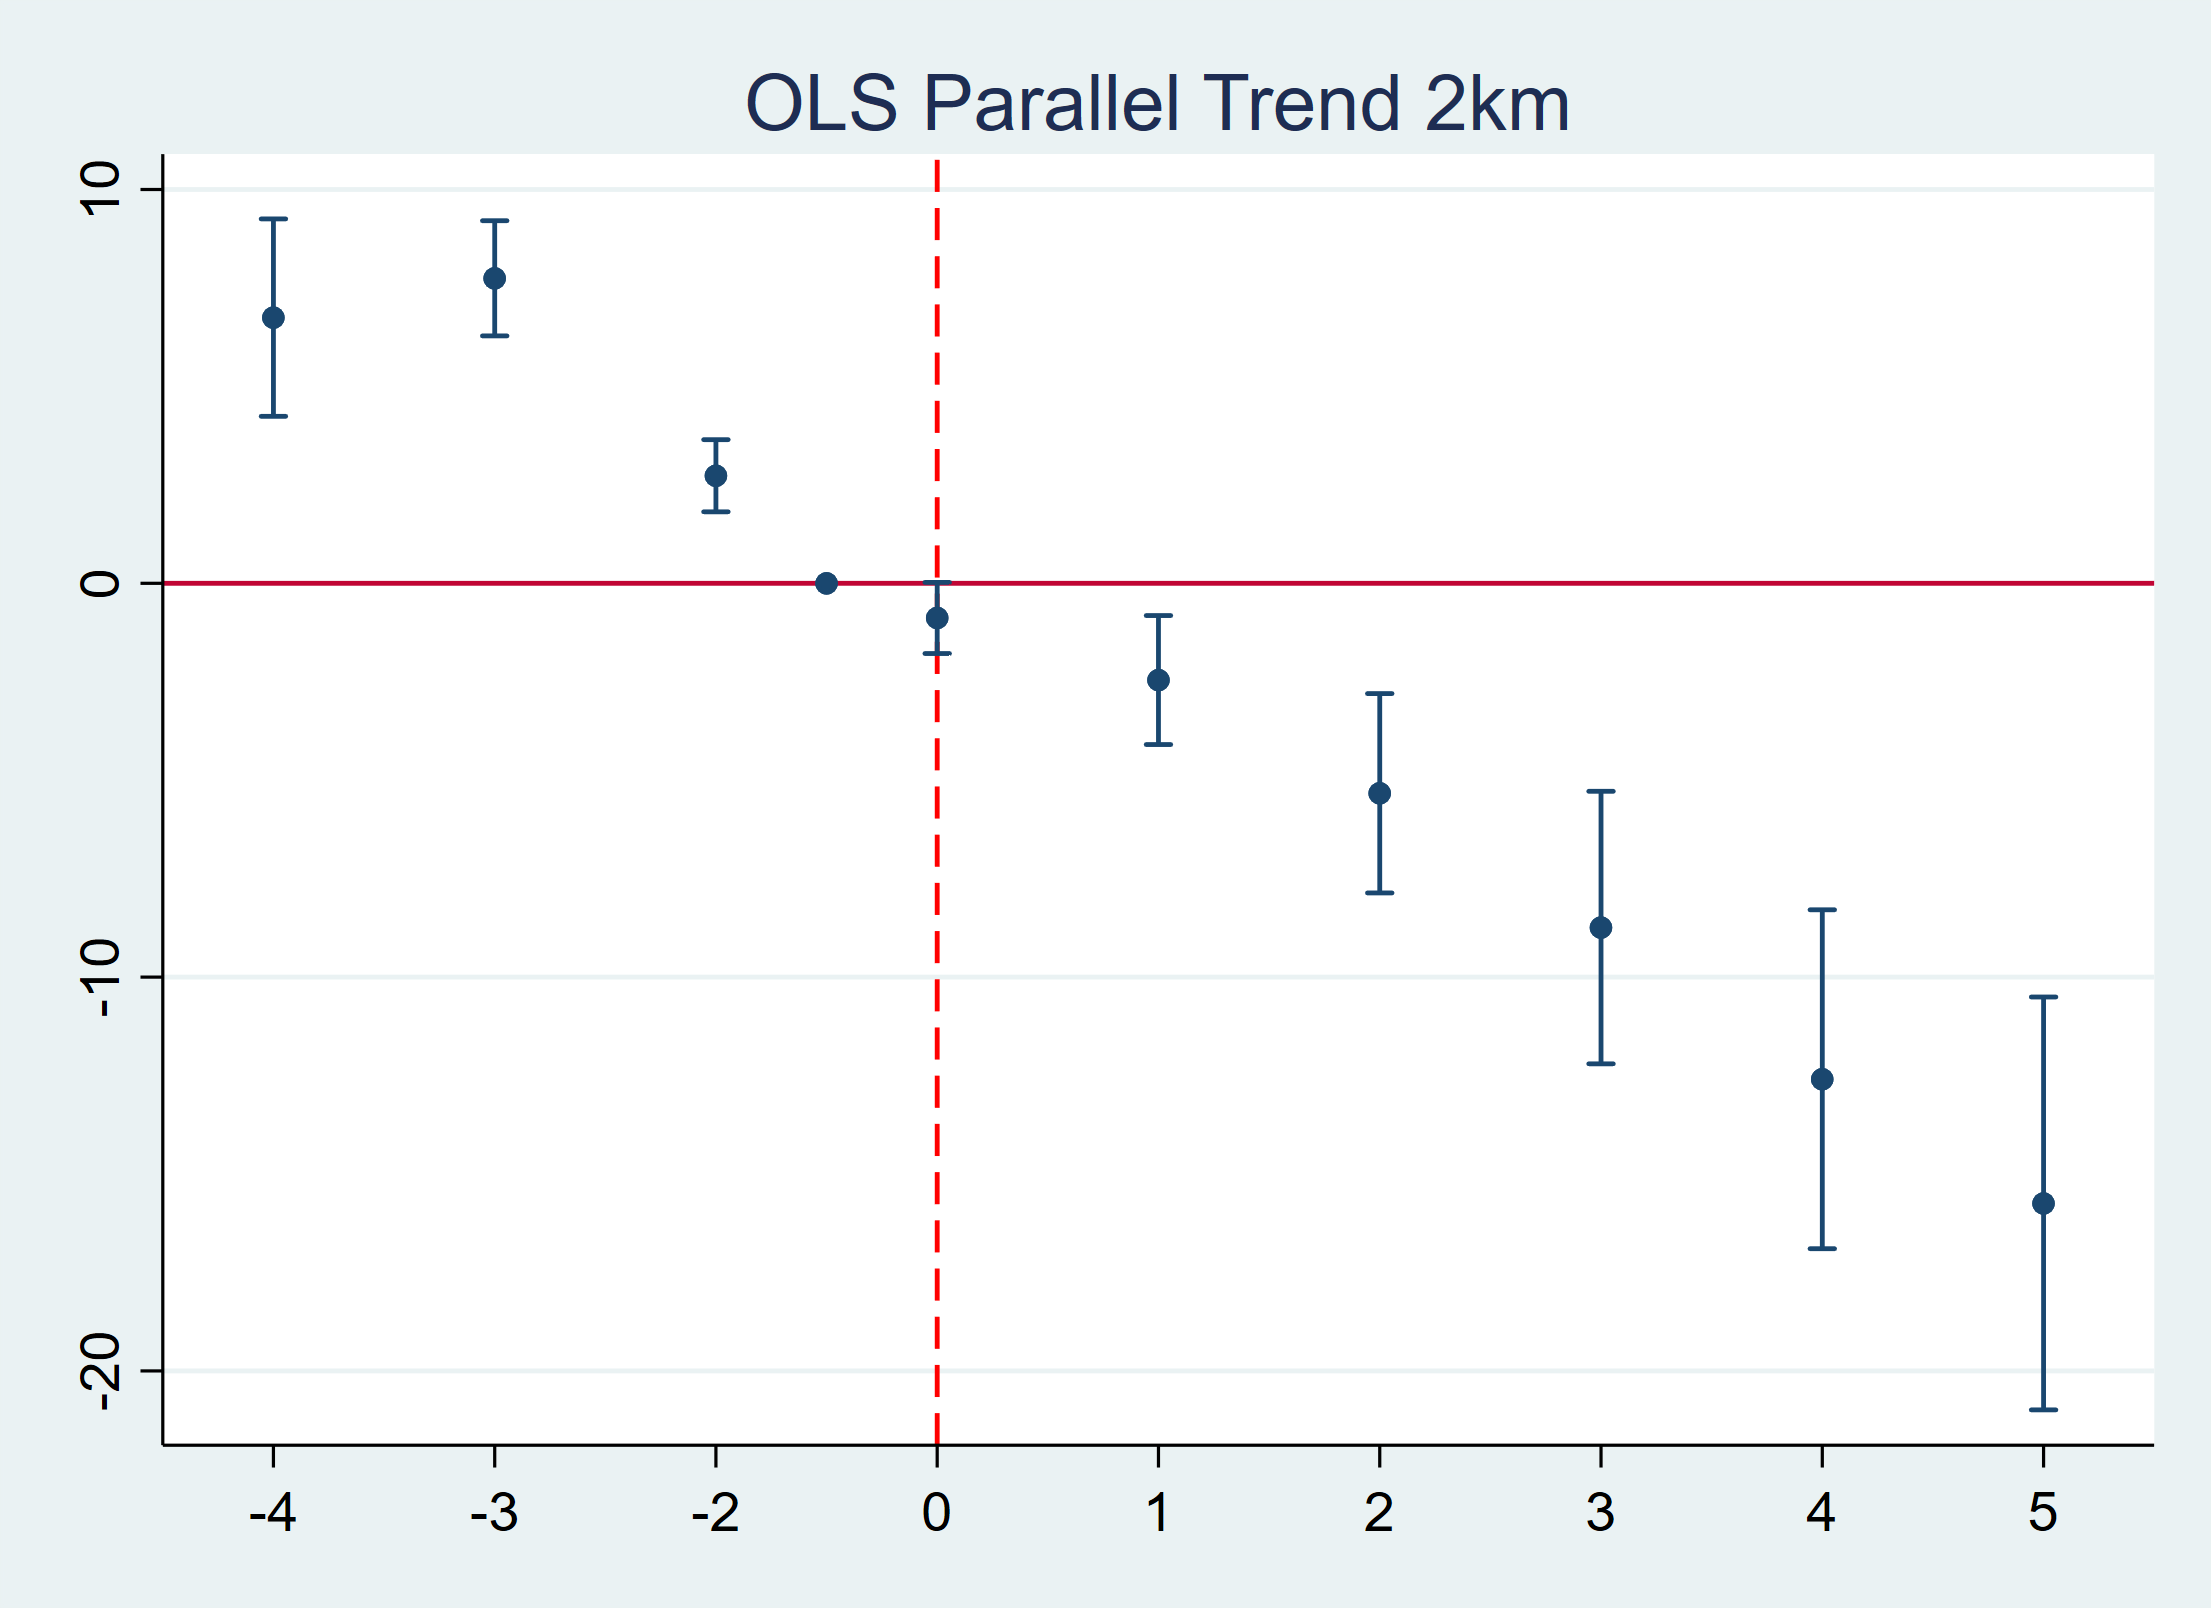
\includegraphics[width=0.8\textwidth]{parallel_ols_2km.png}
\end{center}

\end{frame}


\begin{frame}{Event Study:TWFE}

\begin{itemize}
    \item Outcome: Pharmacy entry around hospitals (within 3km)
    \item Fixed effects: hospital and year
    \item Standard errors : clustered at  county level
\end{itemize}

\vspace{0.5em}
\begin{center}
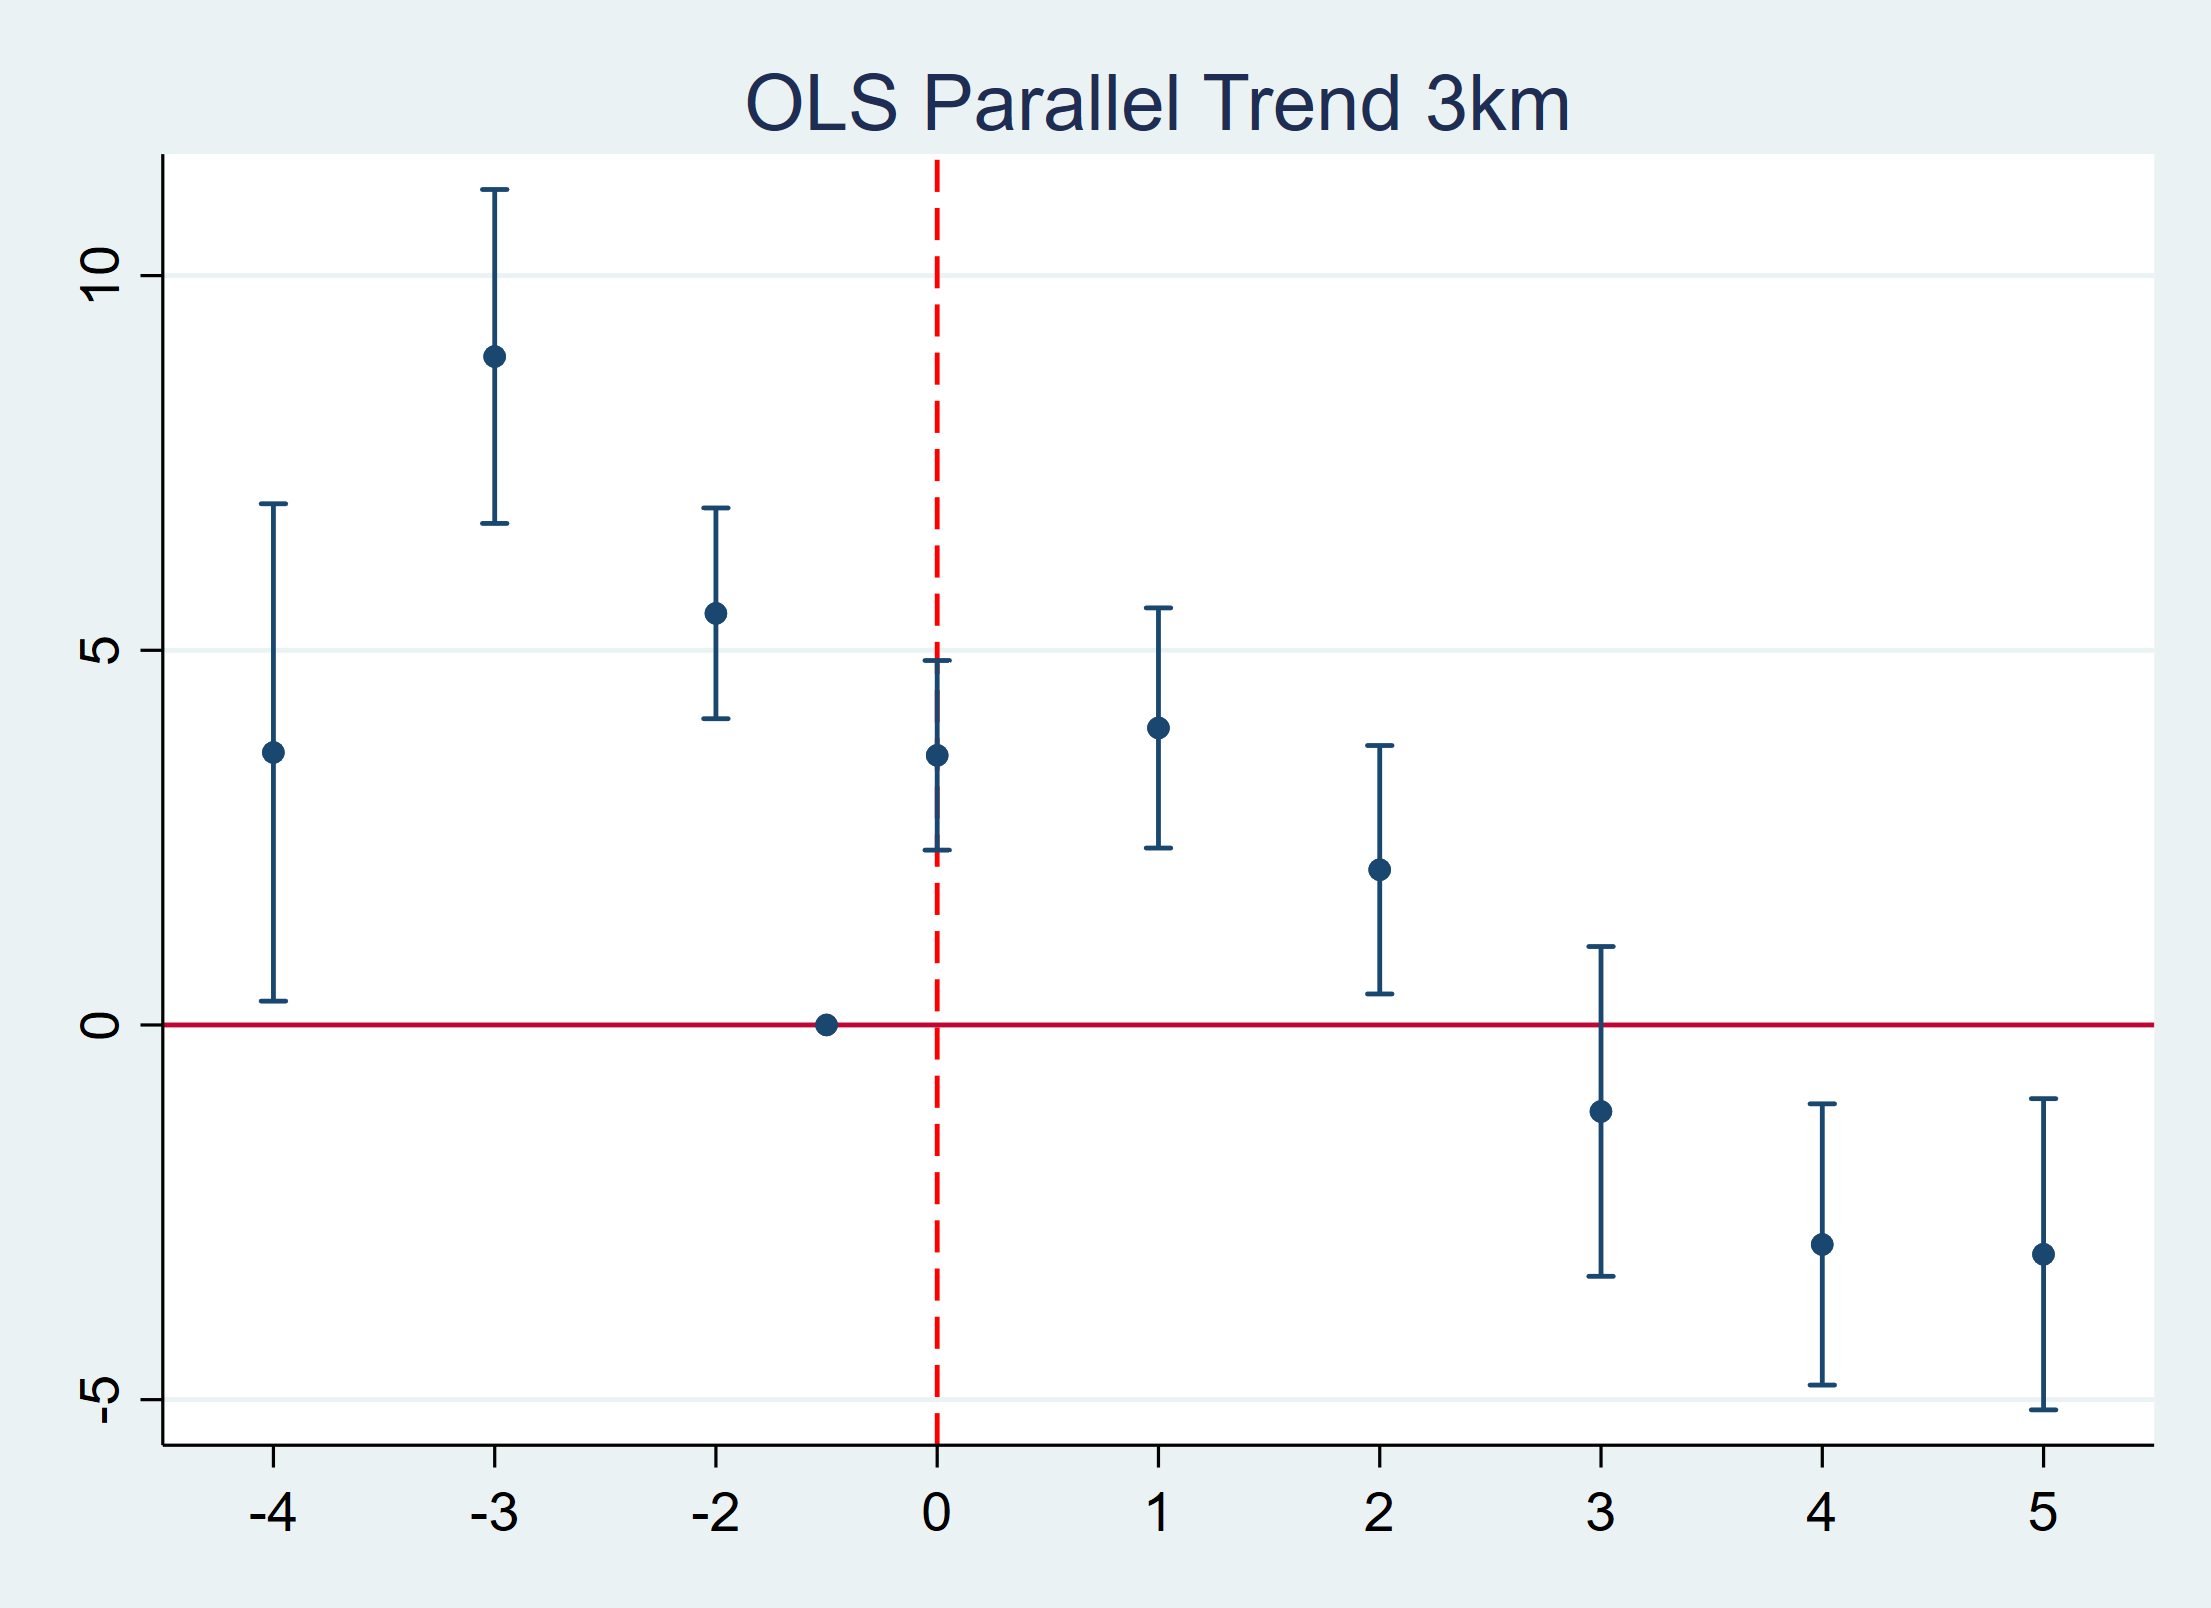
\includegraphics[width=0.8\textwidth]{parallel_ols_3km.png}
\end{center}

\end{frame}

% ========== Event Study:Callaway & Sant’Anna==========
\begin{frame}{Event Study:CS}

\begin{itemize}
    \item Outcome: Pharmacy entry around hospitals (within 1km)
    \item Fixed effects: hospital and year
    \item Standard errors : clustered at  county level
\end{itemize}

\vspace{0.5em}
\begin{center}
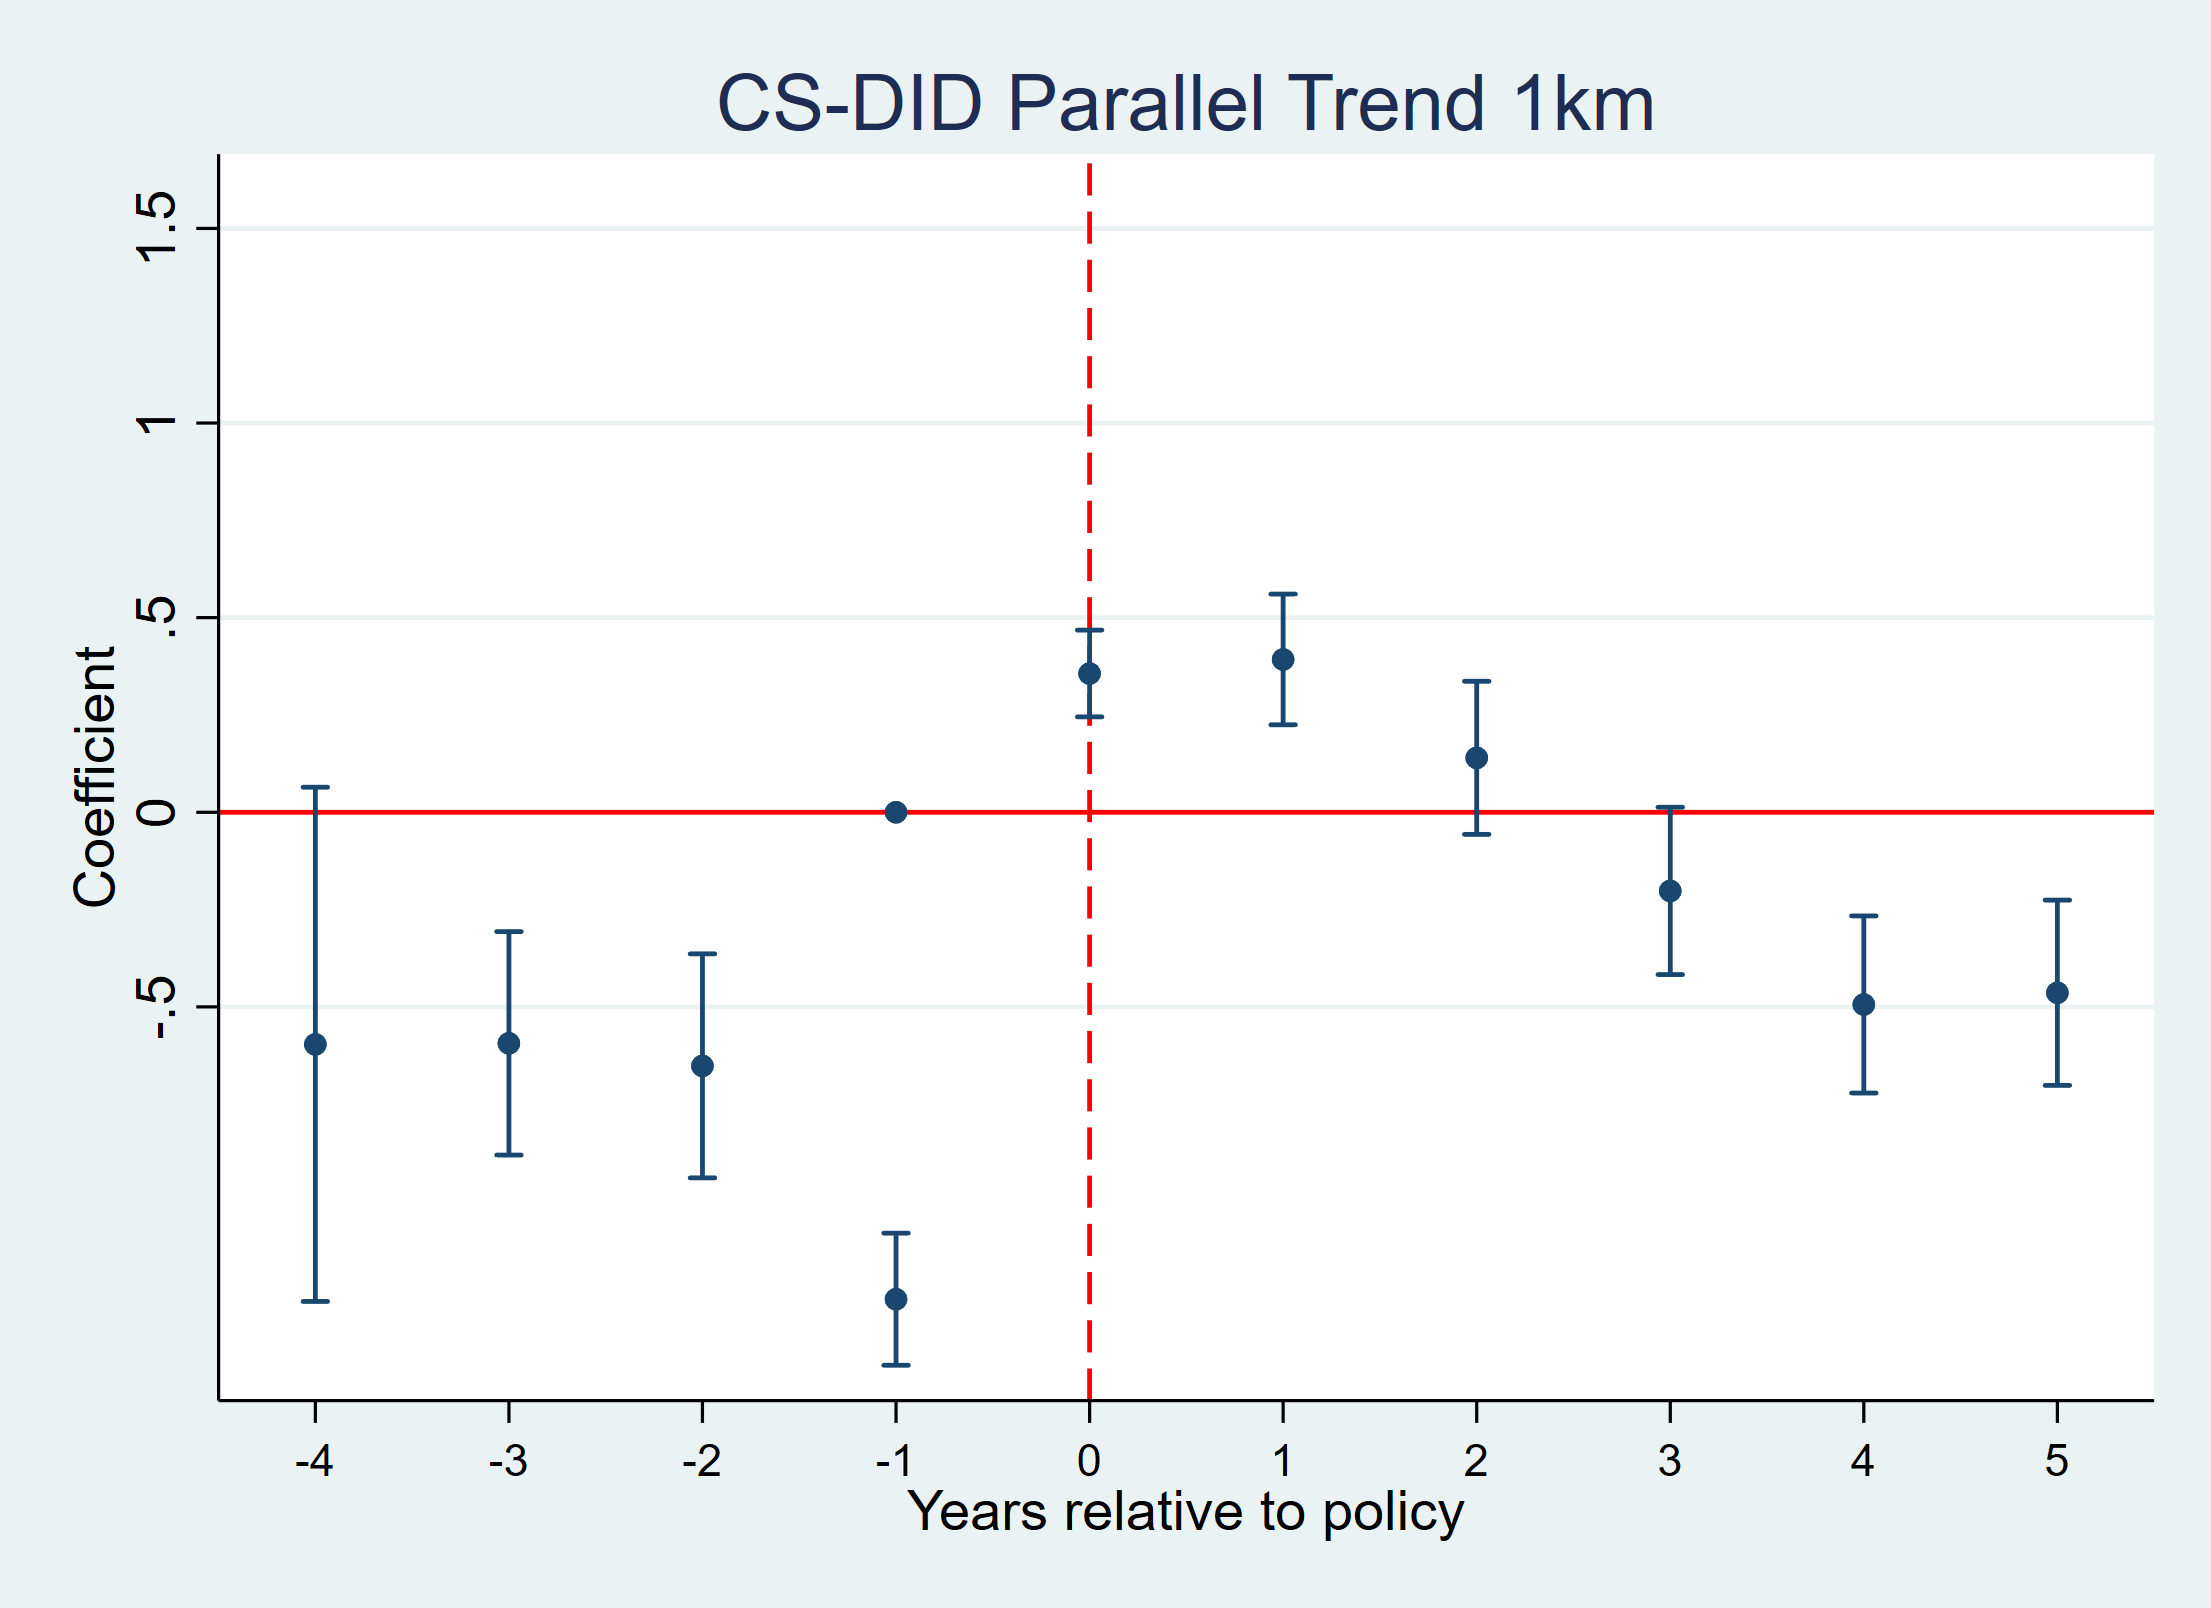
\includegraphics[width=0.8\textwidth]{cs_event_1km.png}
\end{center}

\end{frame}

\begin{frame}{Event Study:CS}

\begin{itemize}
    \item Outcome: Pharmacy entry around hospitals (within 2km)
    \item Fixed effects: hospital and year
    \item Standard errors : clustered at  county level
\end{itemize}

\vspace{0.5em}
\begin{center}
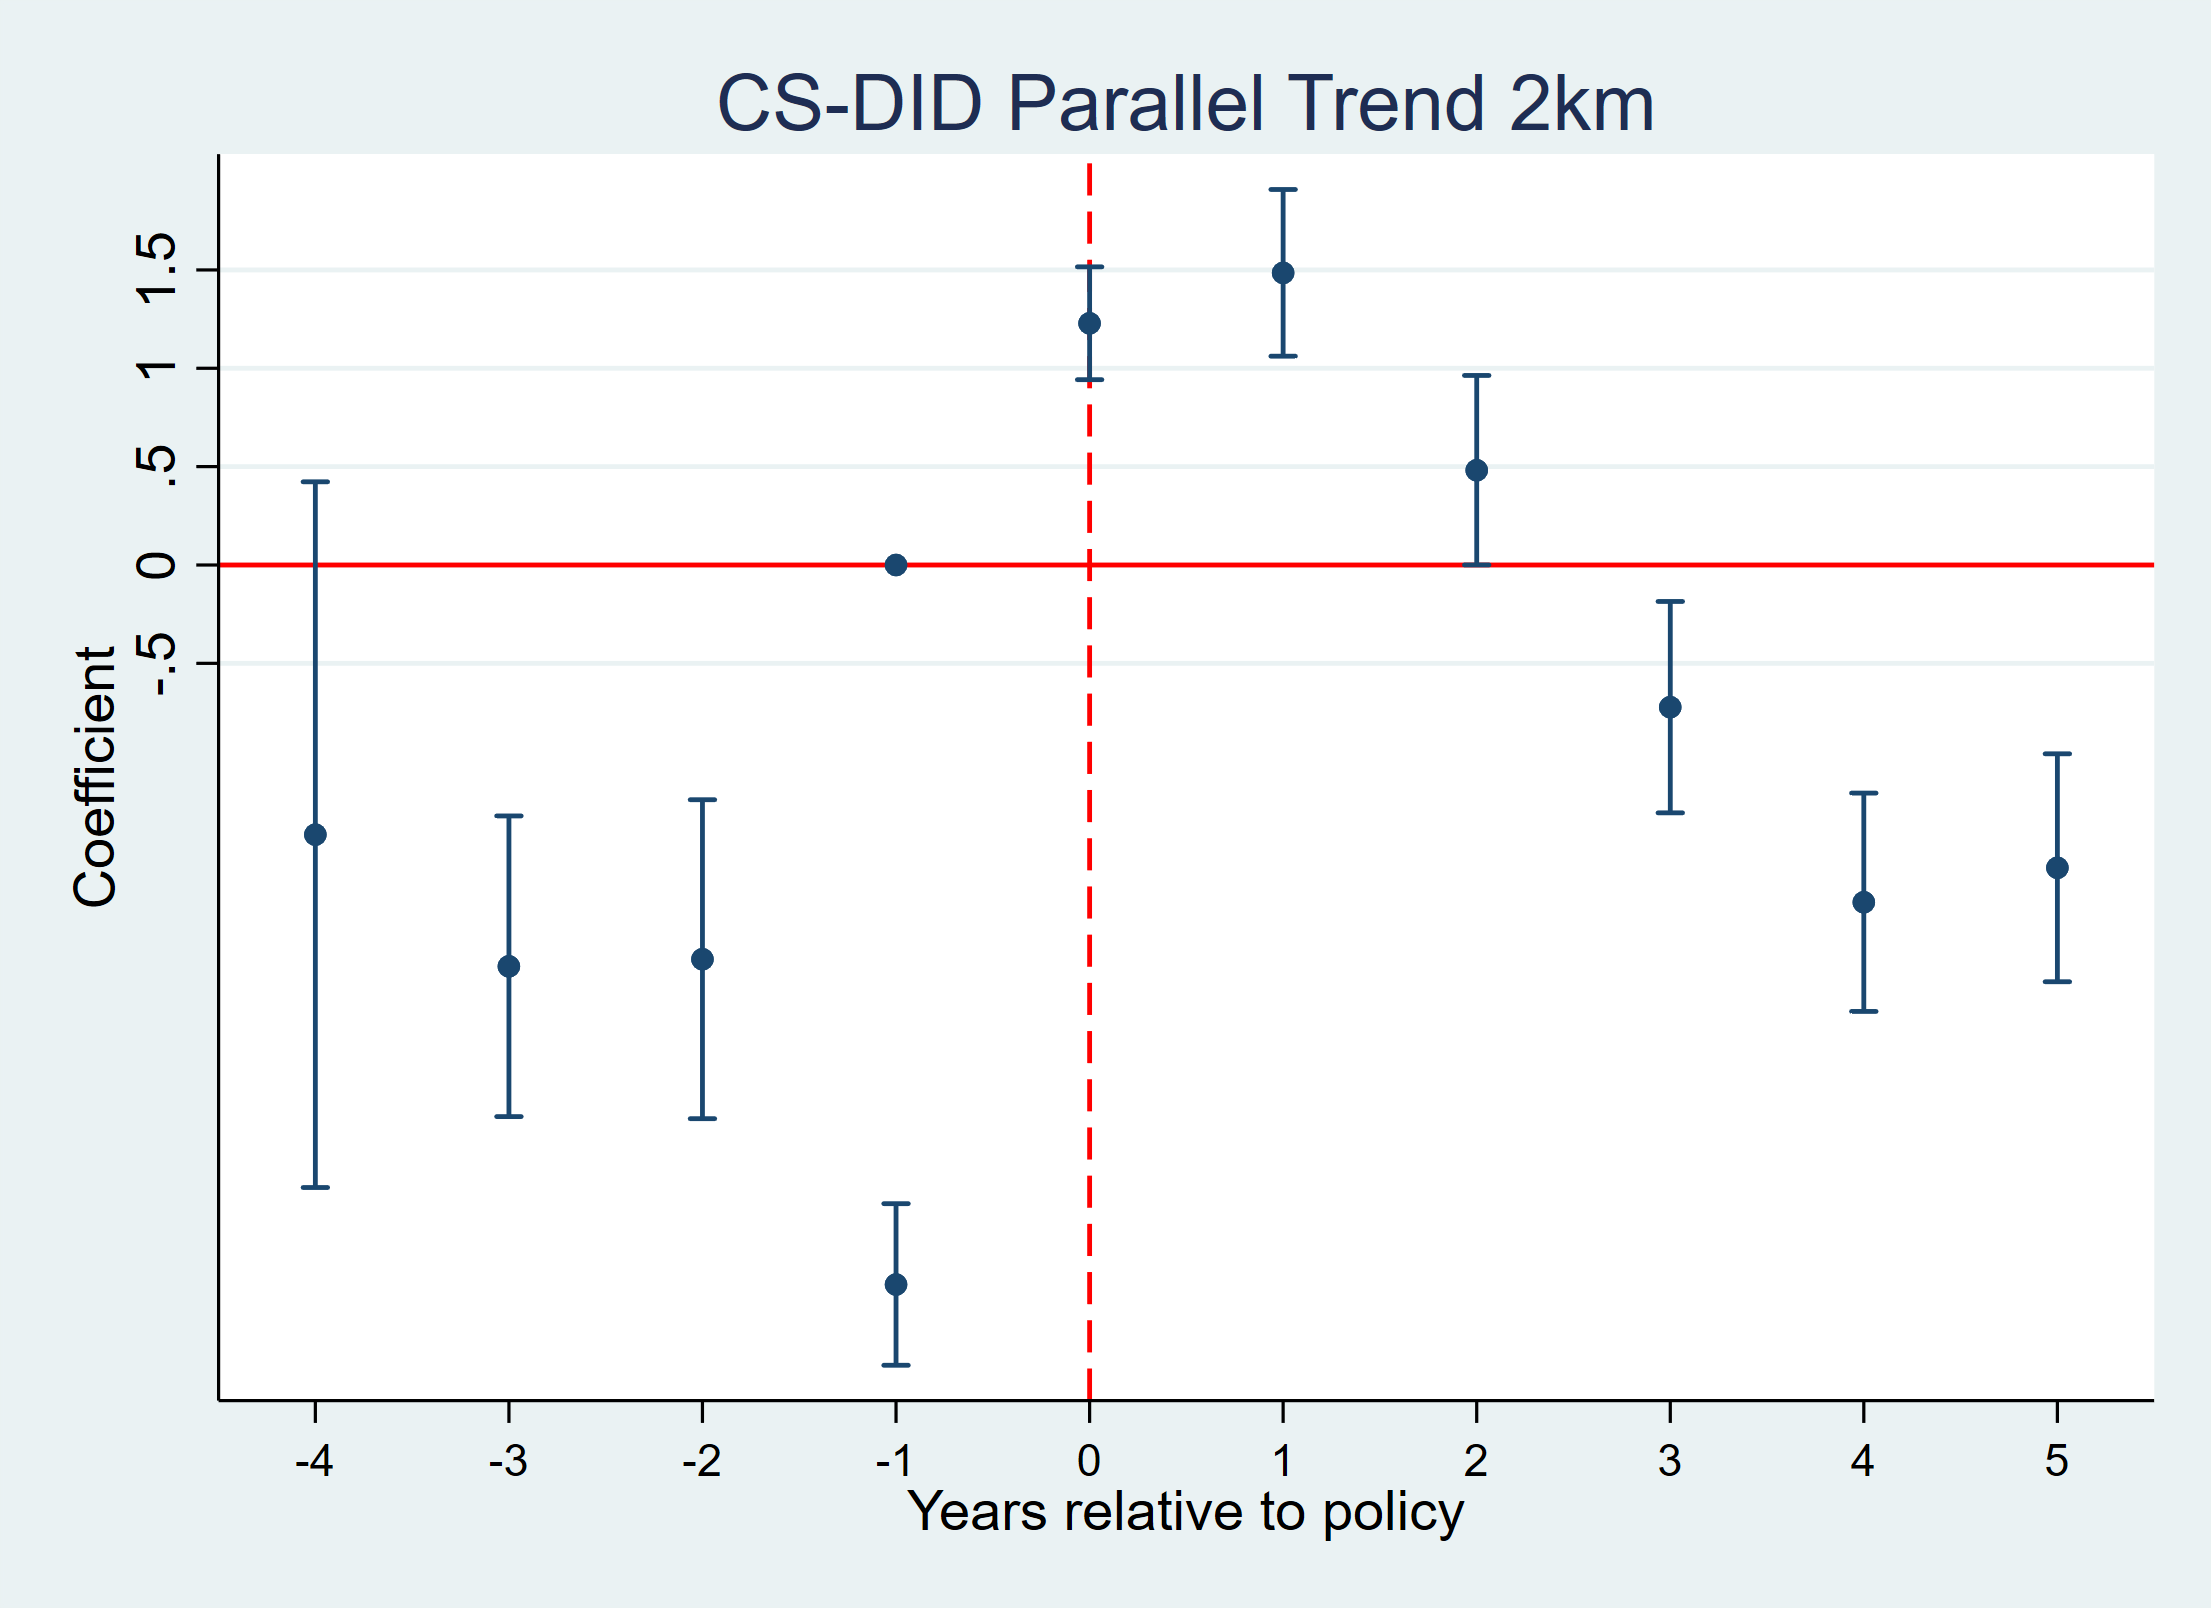
\includegraphics[width=0.8\textwidth]{cs_event_2km.png}
\end{center}

\end{frame}


\begin{frame}{Event Study:CS}

\begin{itemize}
    \item Outcome: Pharmacy entry around hospitals (within 3km)
    \item Fixed effects: hospital and year
    \item Standard errors : clustered at  county level
\end{itemize}

\vspace{0.5em}
\begin{center}
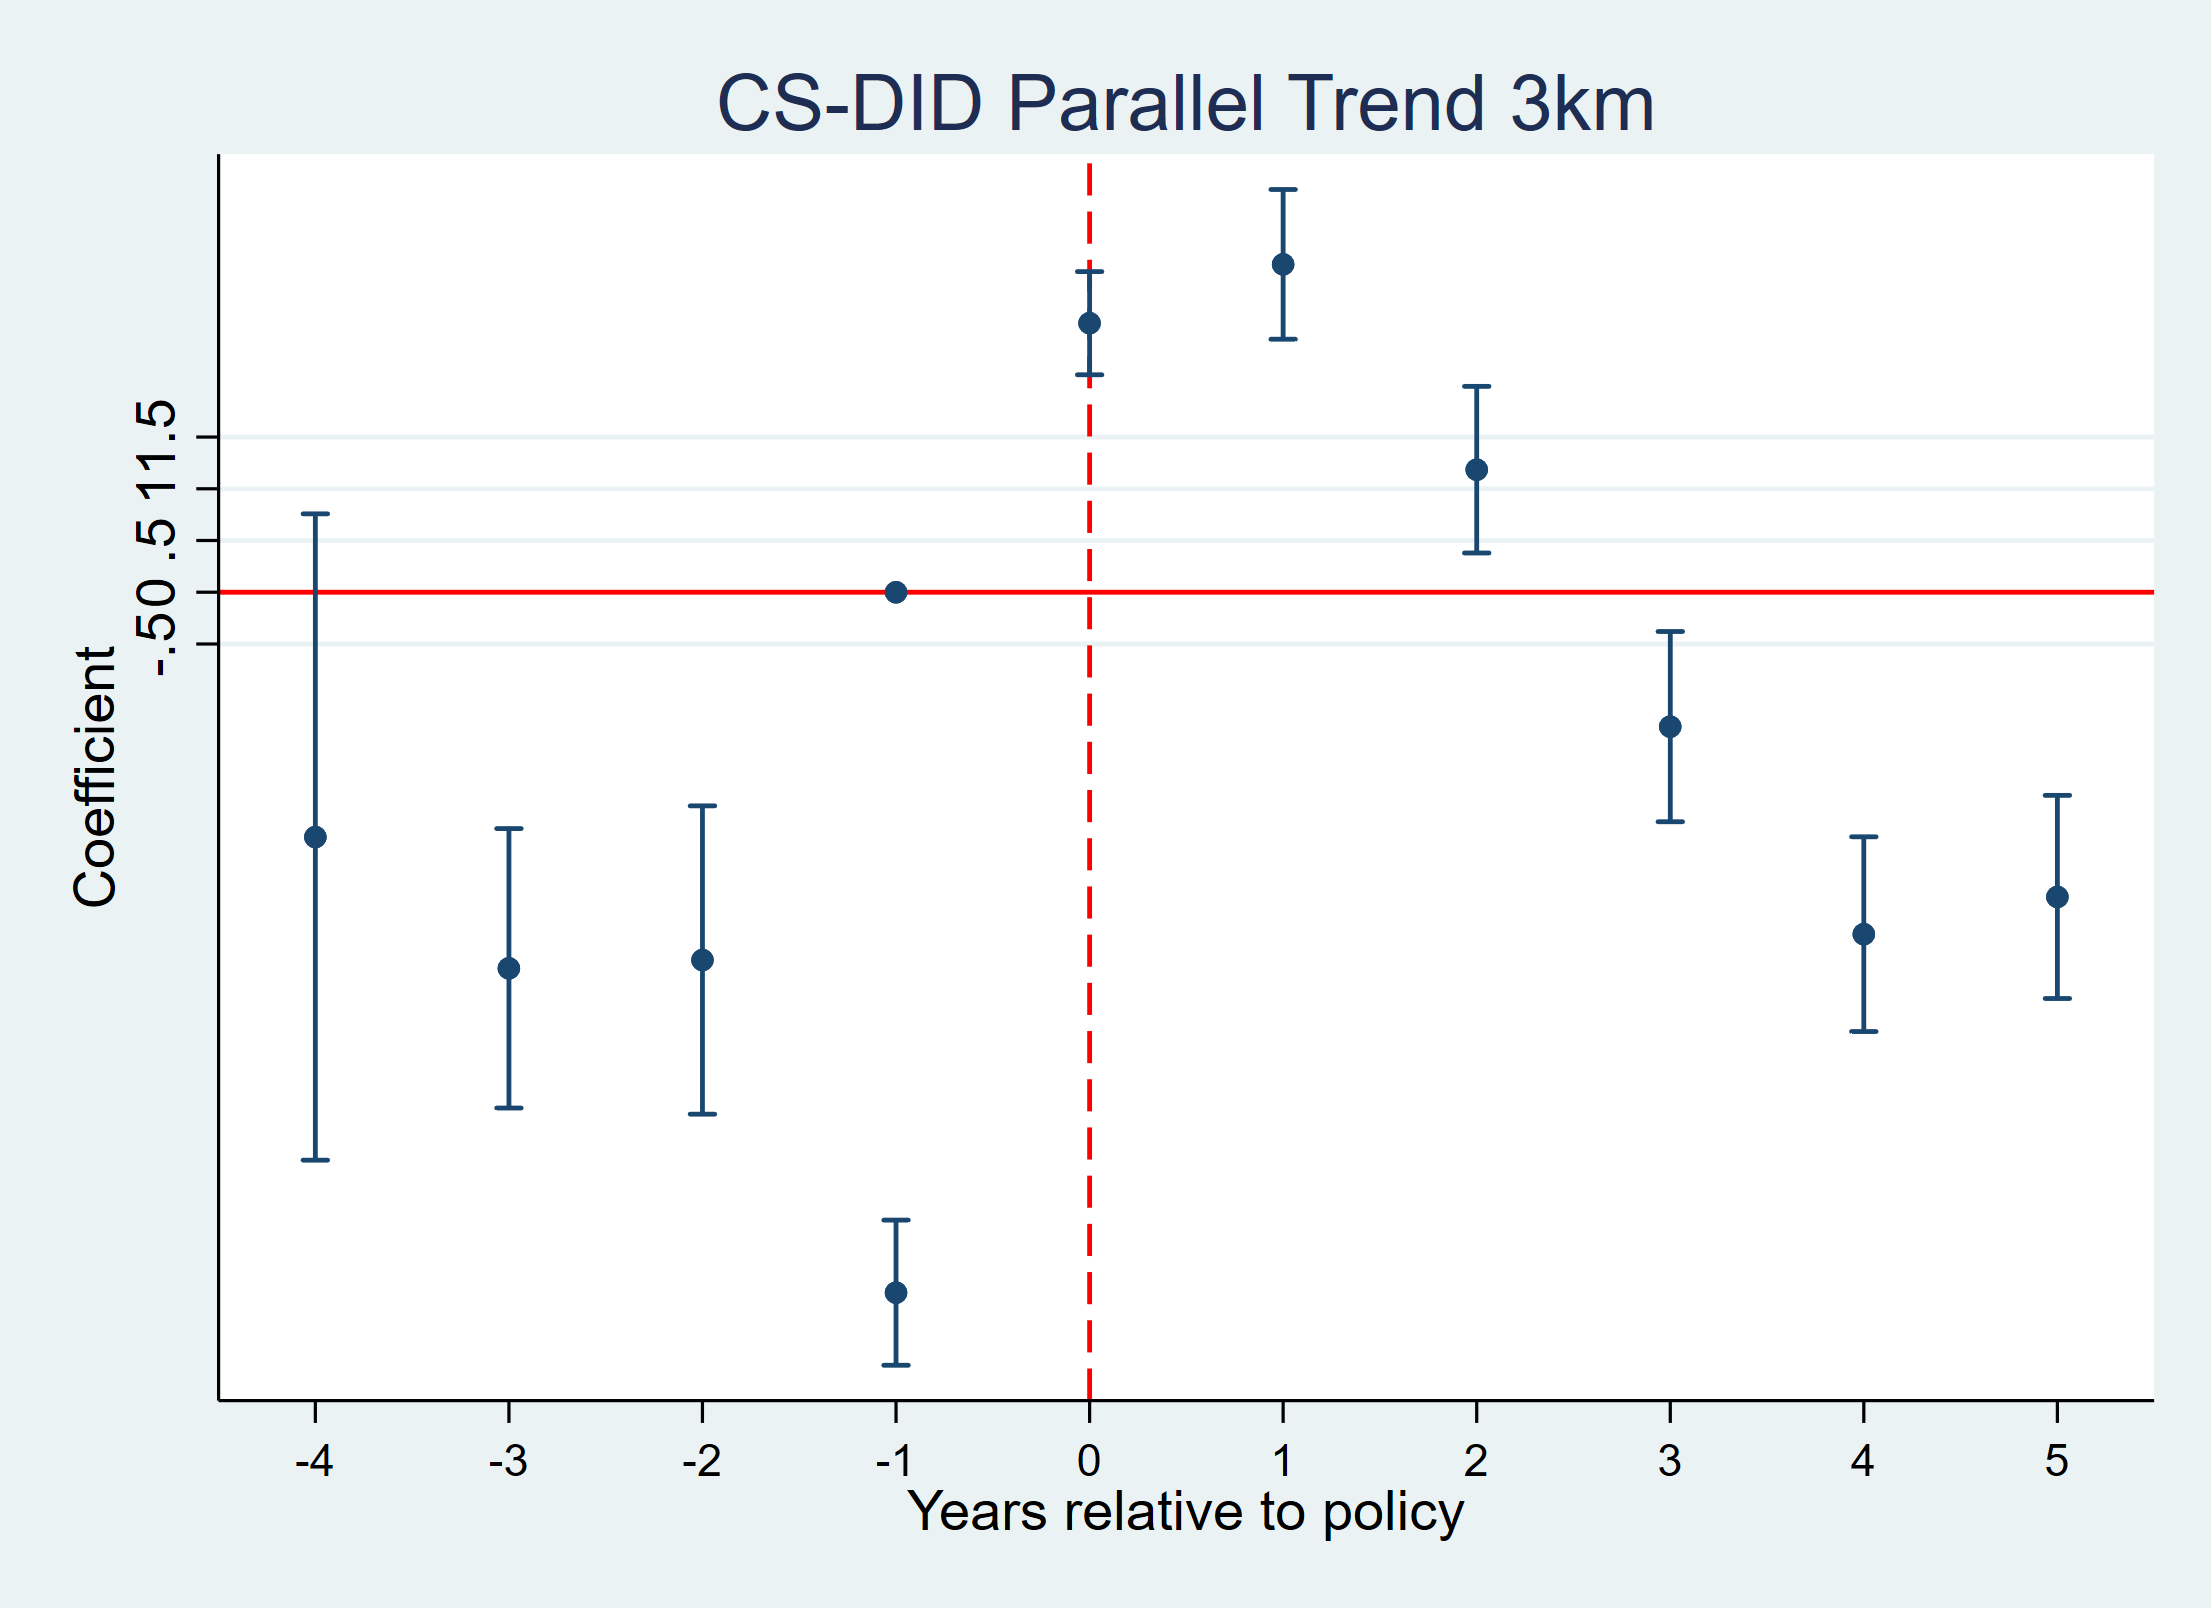
\includegraphics[width=0.8\textwidth]{cs_event_3km.png}
\end{center}

\end{frame}


\begin{frame}{Event Study:CS +trend}

\begin{itemize}
    \item Outcome: Pharmacy entry around hospitals (within 1km)
    \item Fixed effects: hospital and year
    \item trend : county year trend
    \item Standard errors : clustered at  county level
\end{itemize}

\vspace{0.5em}
\begin{center}
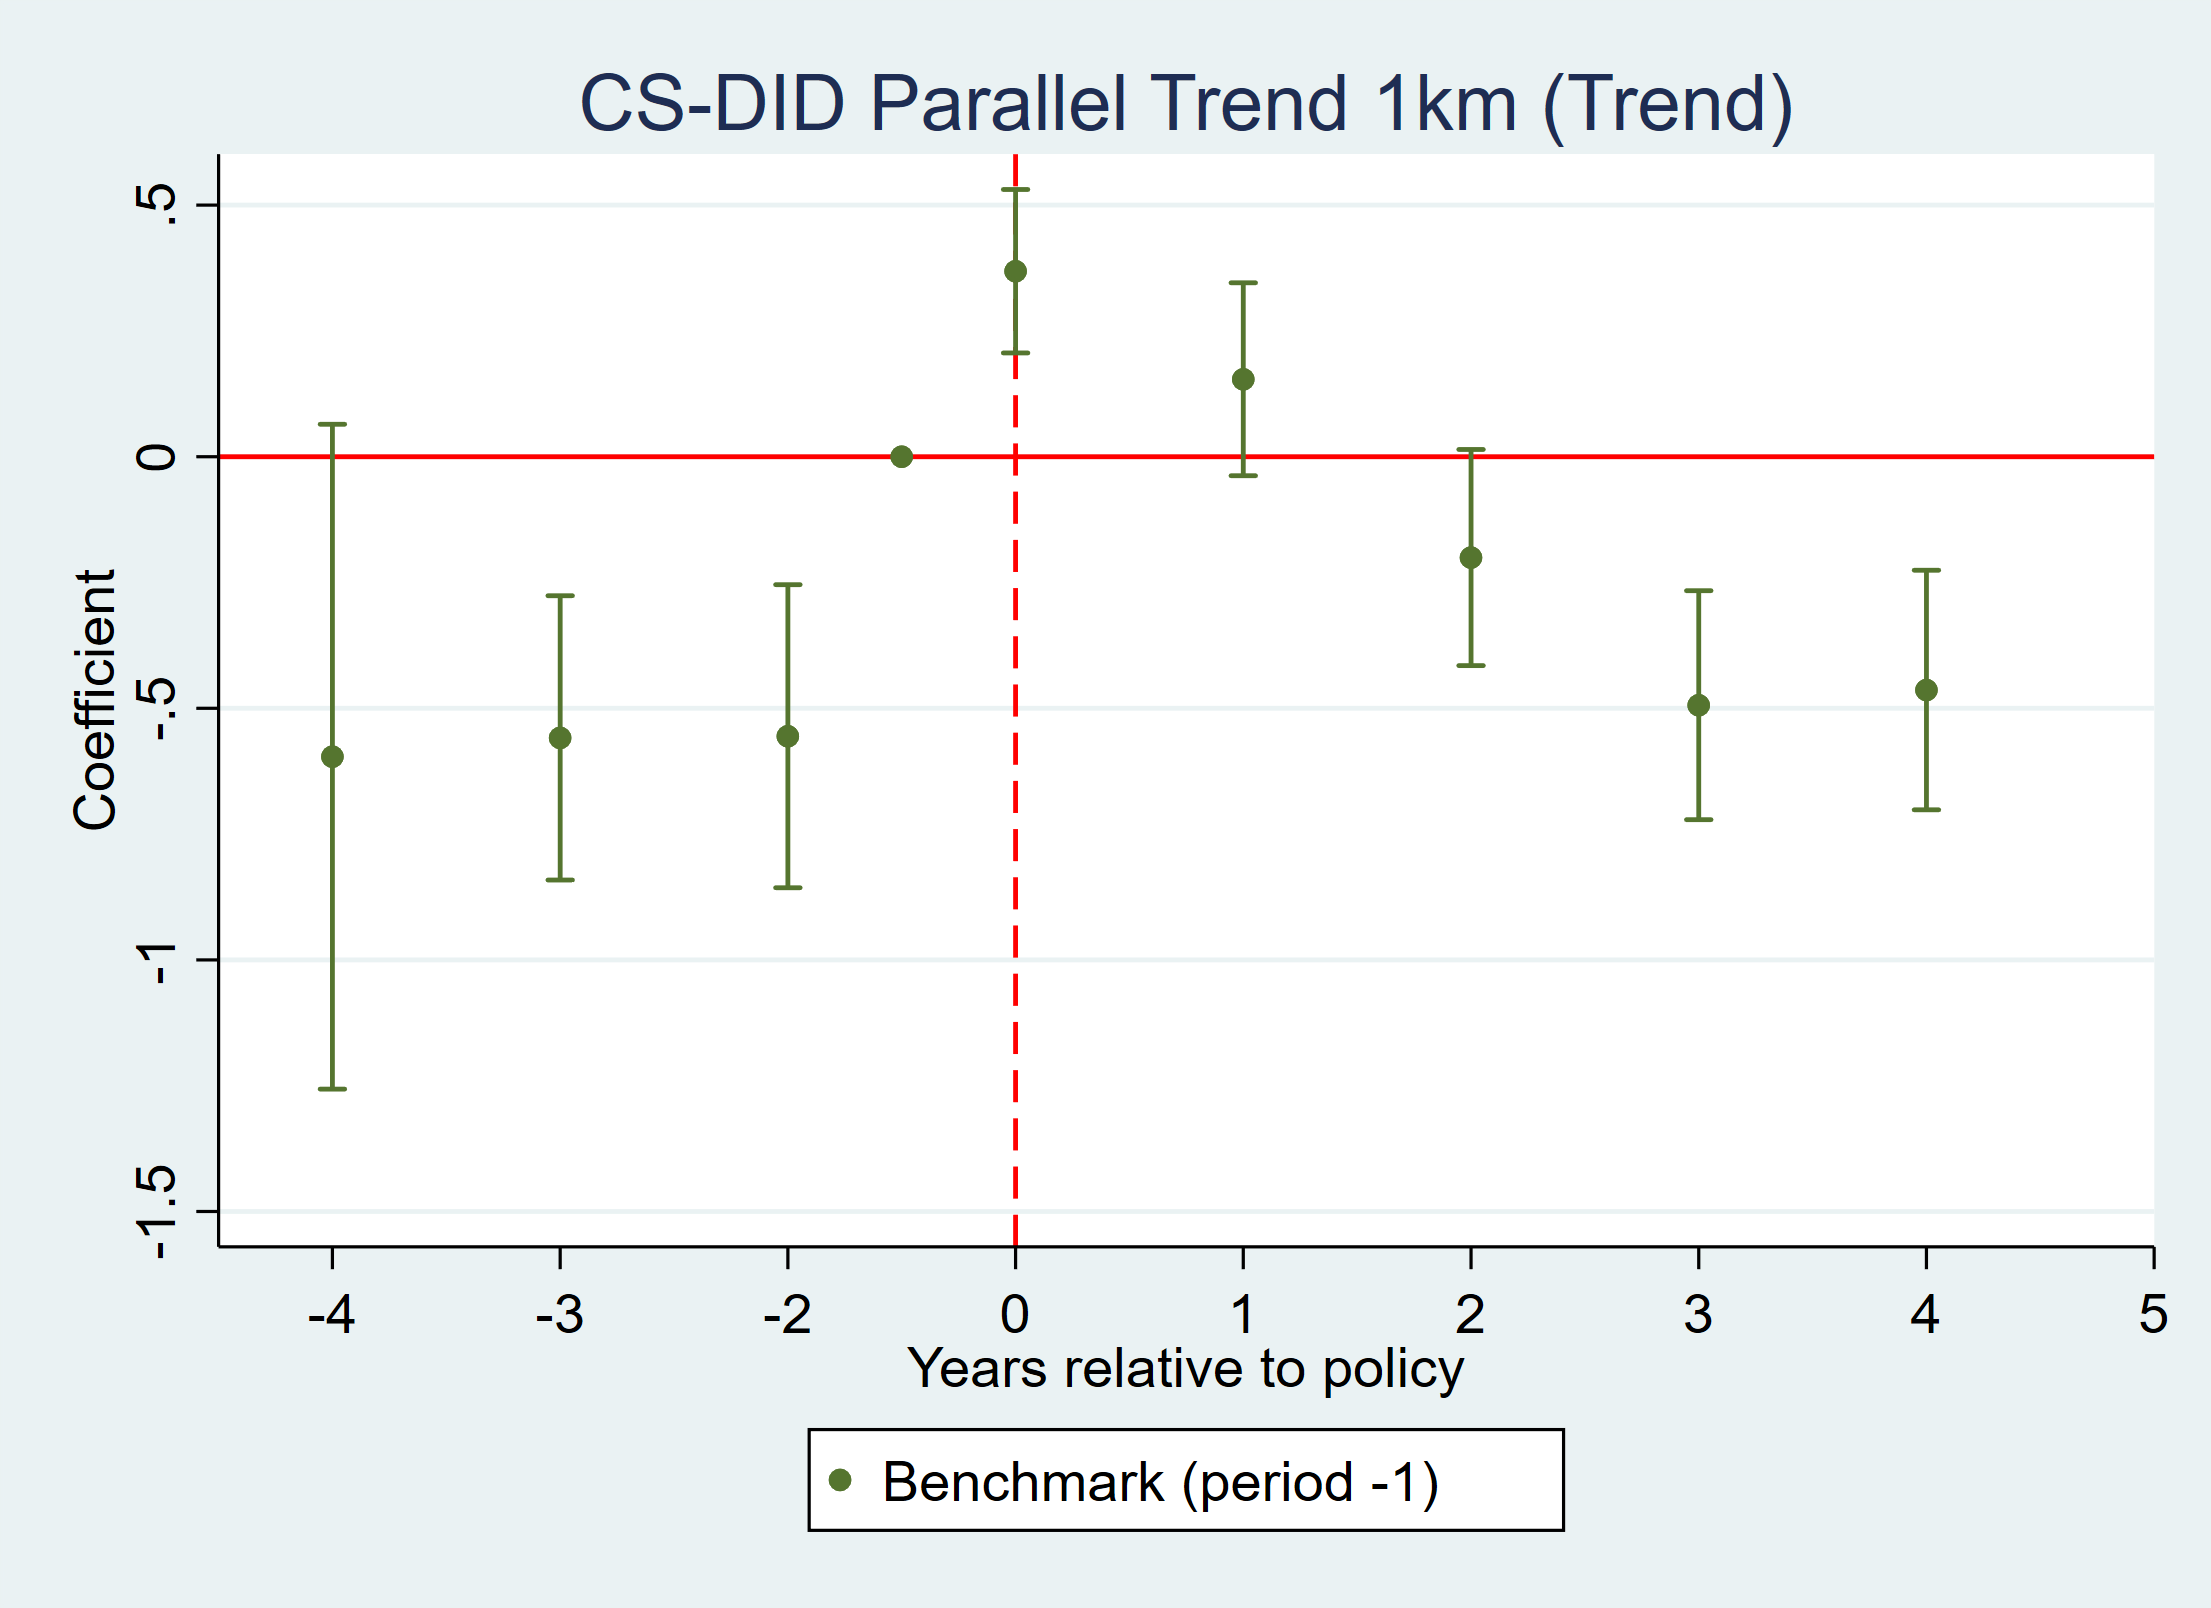
\includegraphics[width=0.8\textwidth]{cs_trend_1km.png}
\end{center}

\end{frame}

\begin{frame}{Event Study:CS +trend}

\begin{itemize}
    \item Outcome: Pharmacy entry around hospitals (within 2km)
    \item Fixed effects: hospital and year
    \item trend : county year trend
    \item Standard errors : clustered at  county level
\end{itemize}

\vspace{0.5em}
\begin{center}
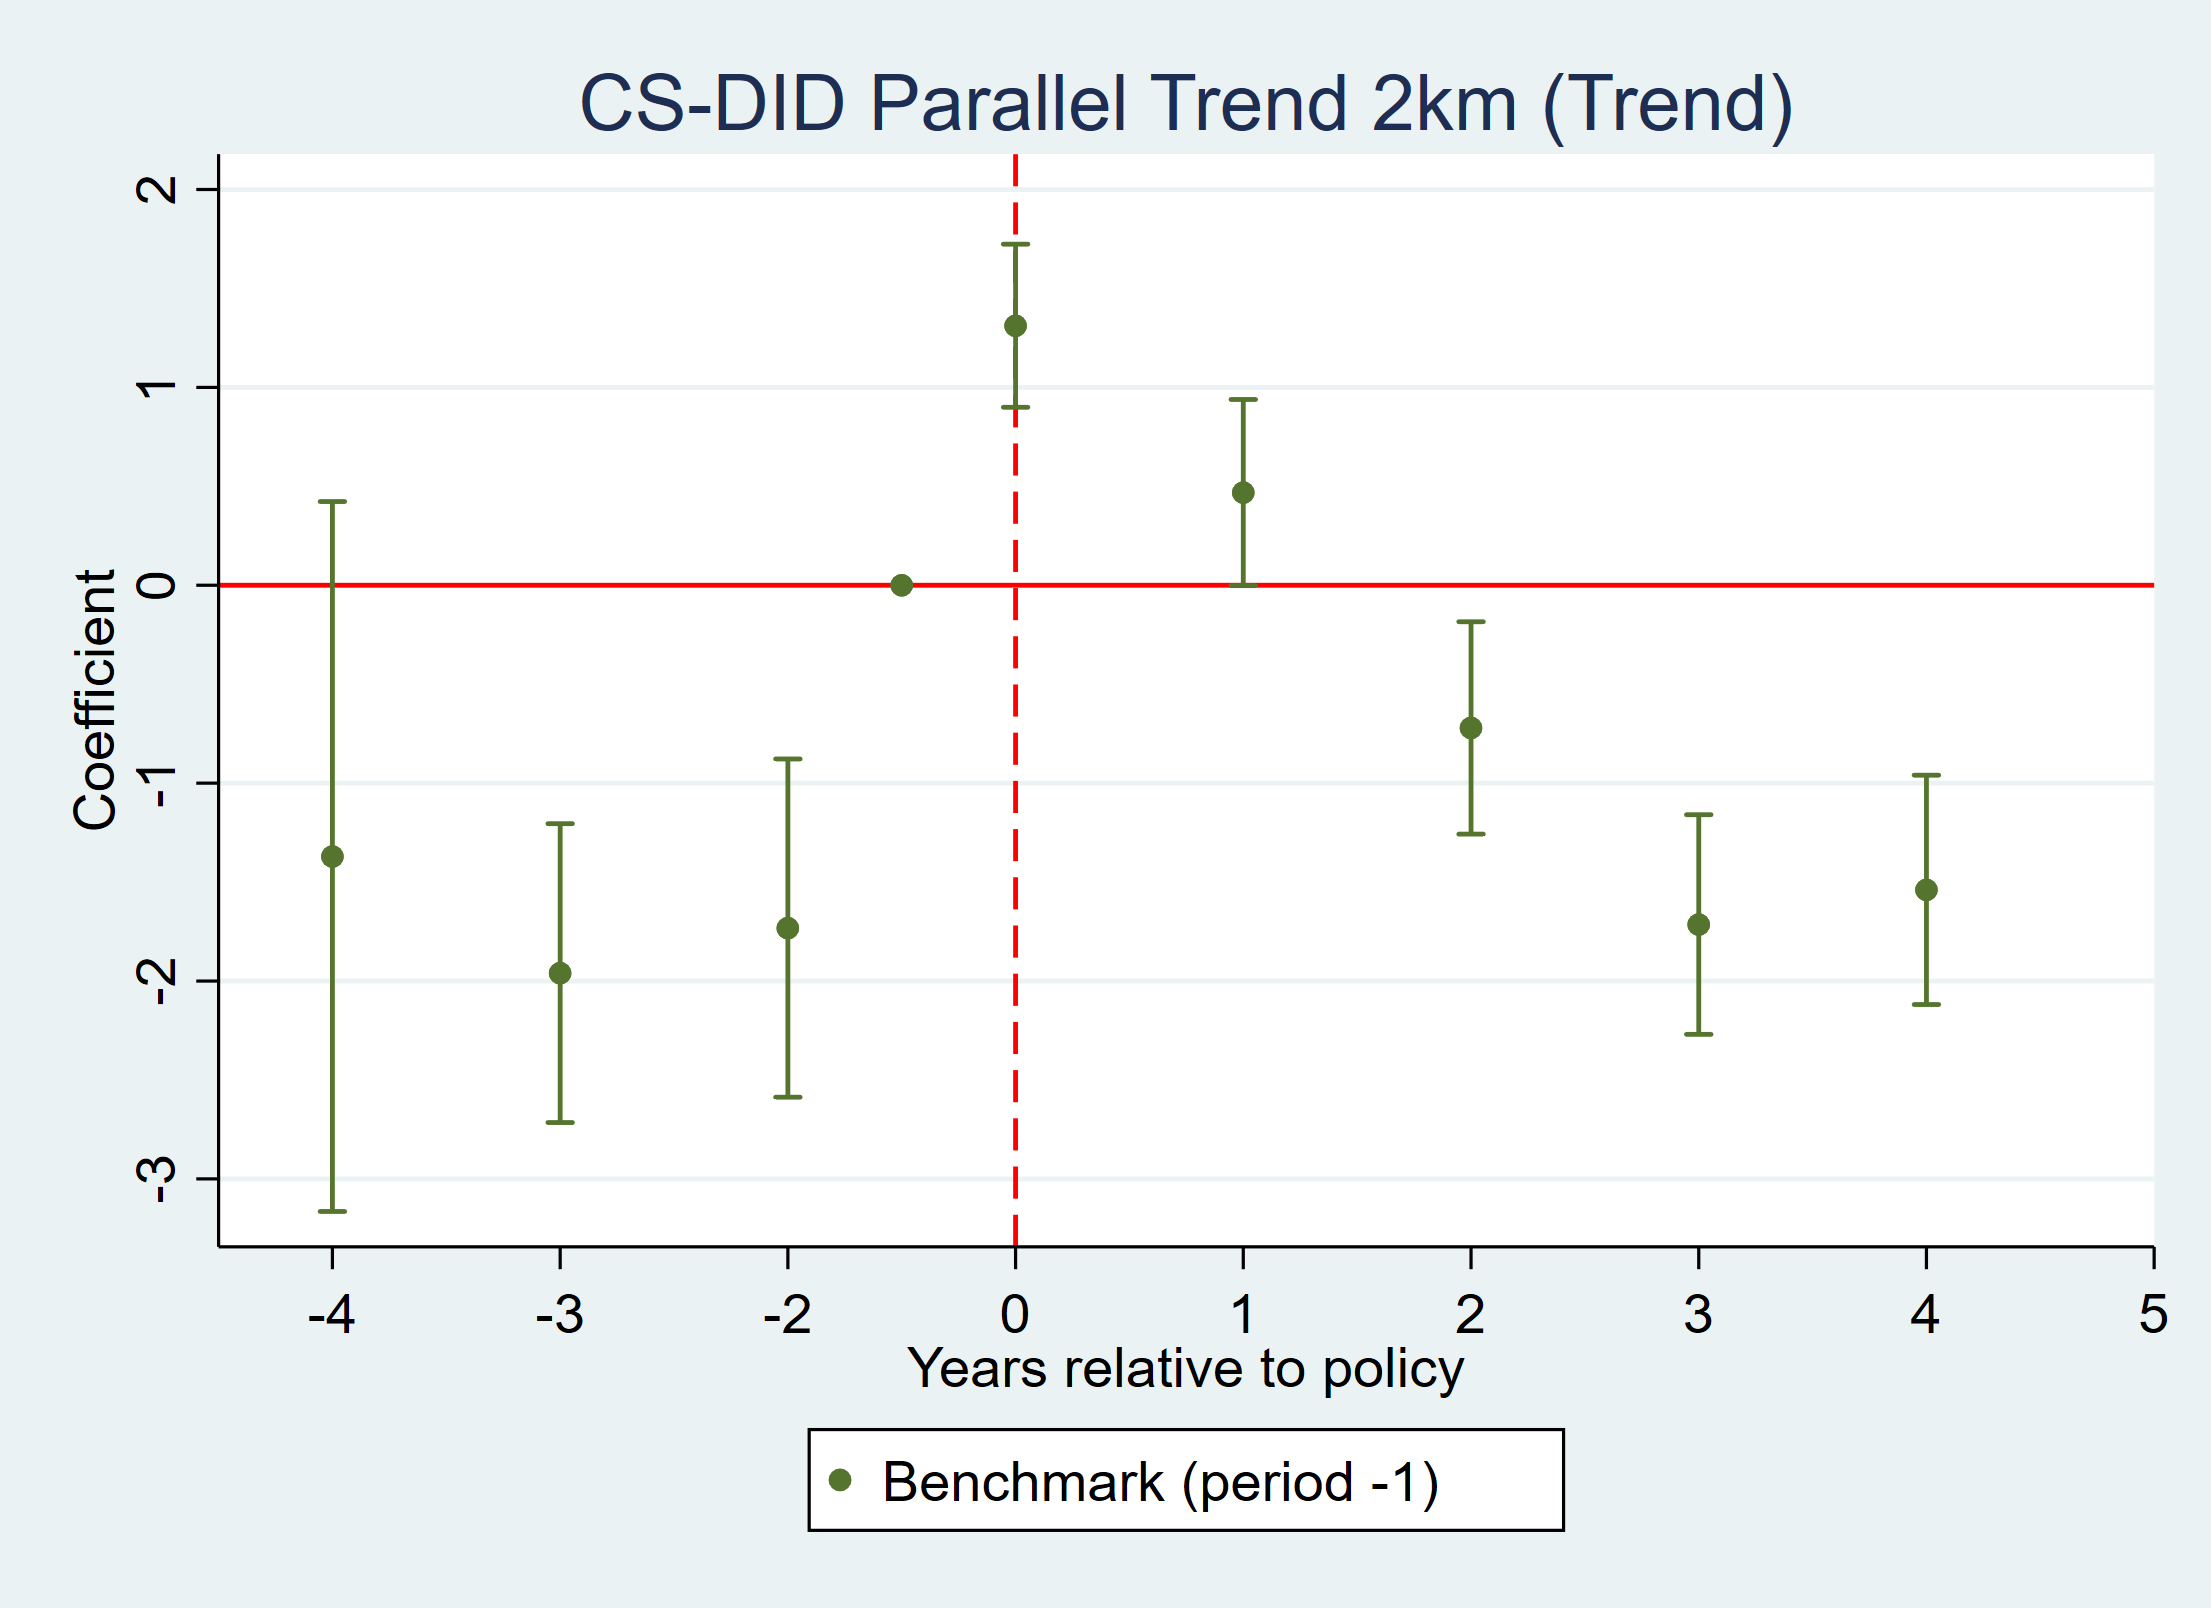
\includegraphics[width=0.8\textwidth]{cs_trend_2km.png}
\end{center}

\end{frame}

\begin{frame}{Event Study:CS +trend}

\begin{itemize}
    \item Outcome: Pharmacy entry around hospitals (within 3km)
    \item Fixed effects: hospital and year 
    \item trend : county year trend
    \item Standard errors : clustered at  county level
\end{itemize}

\vspace{0.5em}
\begin{center}
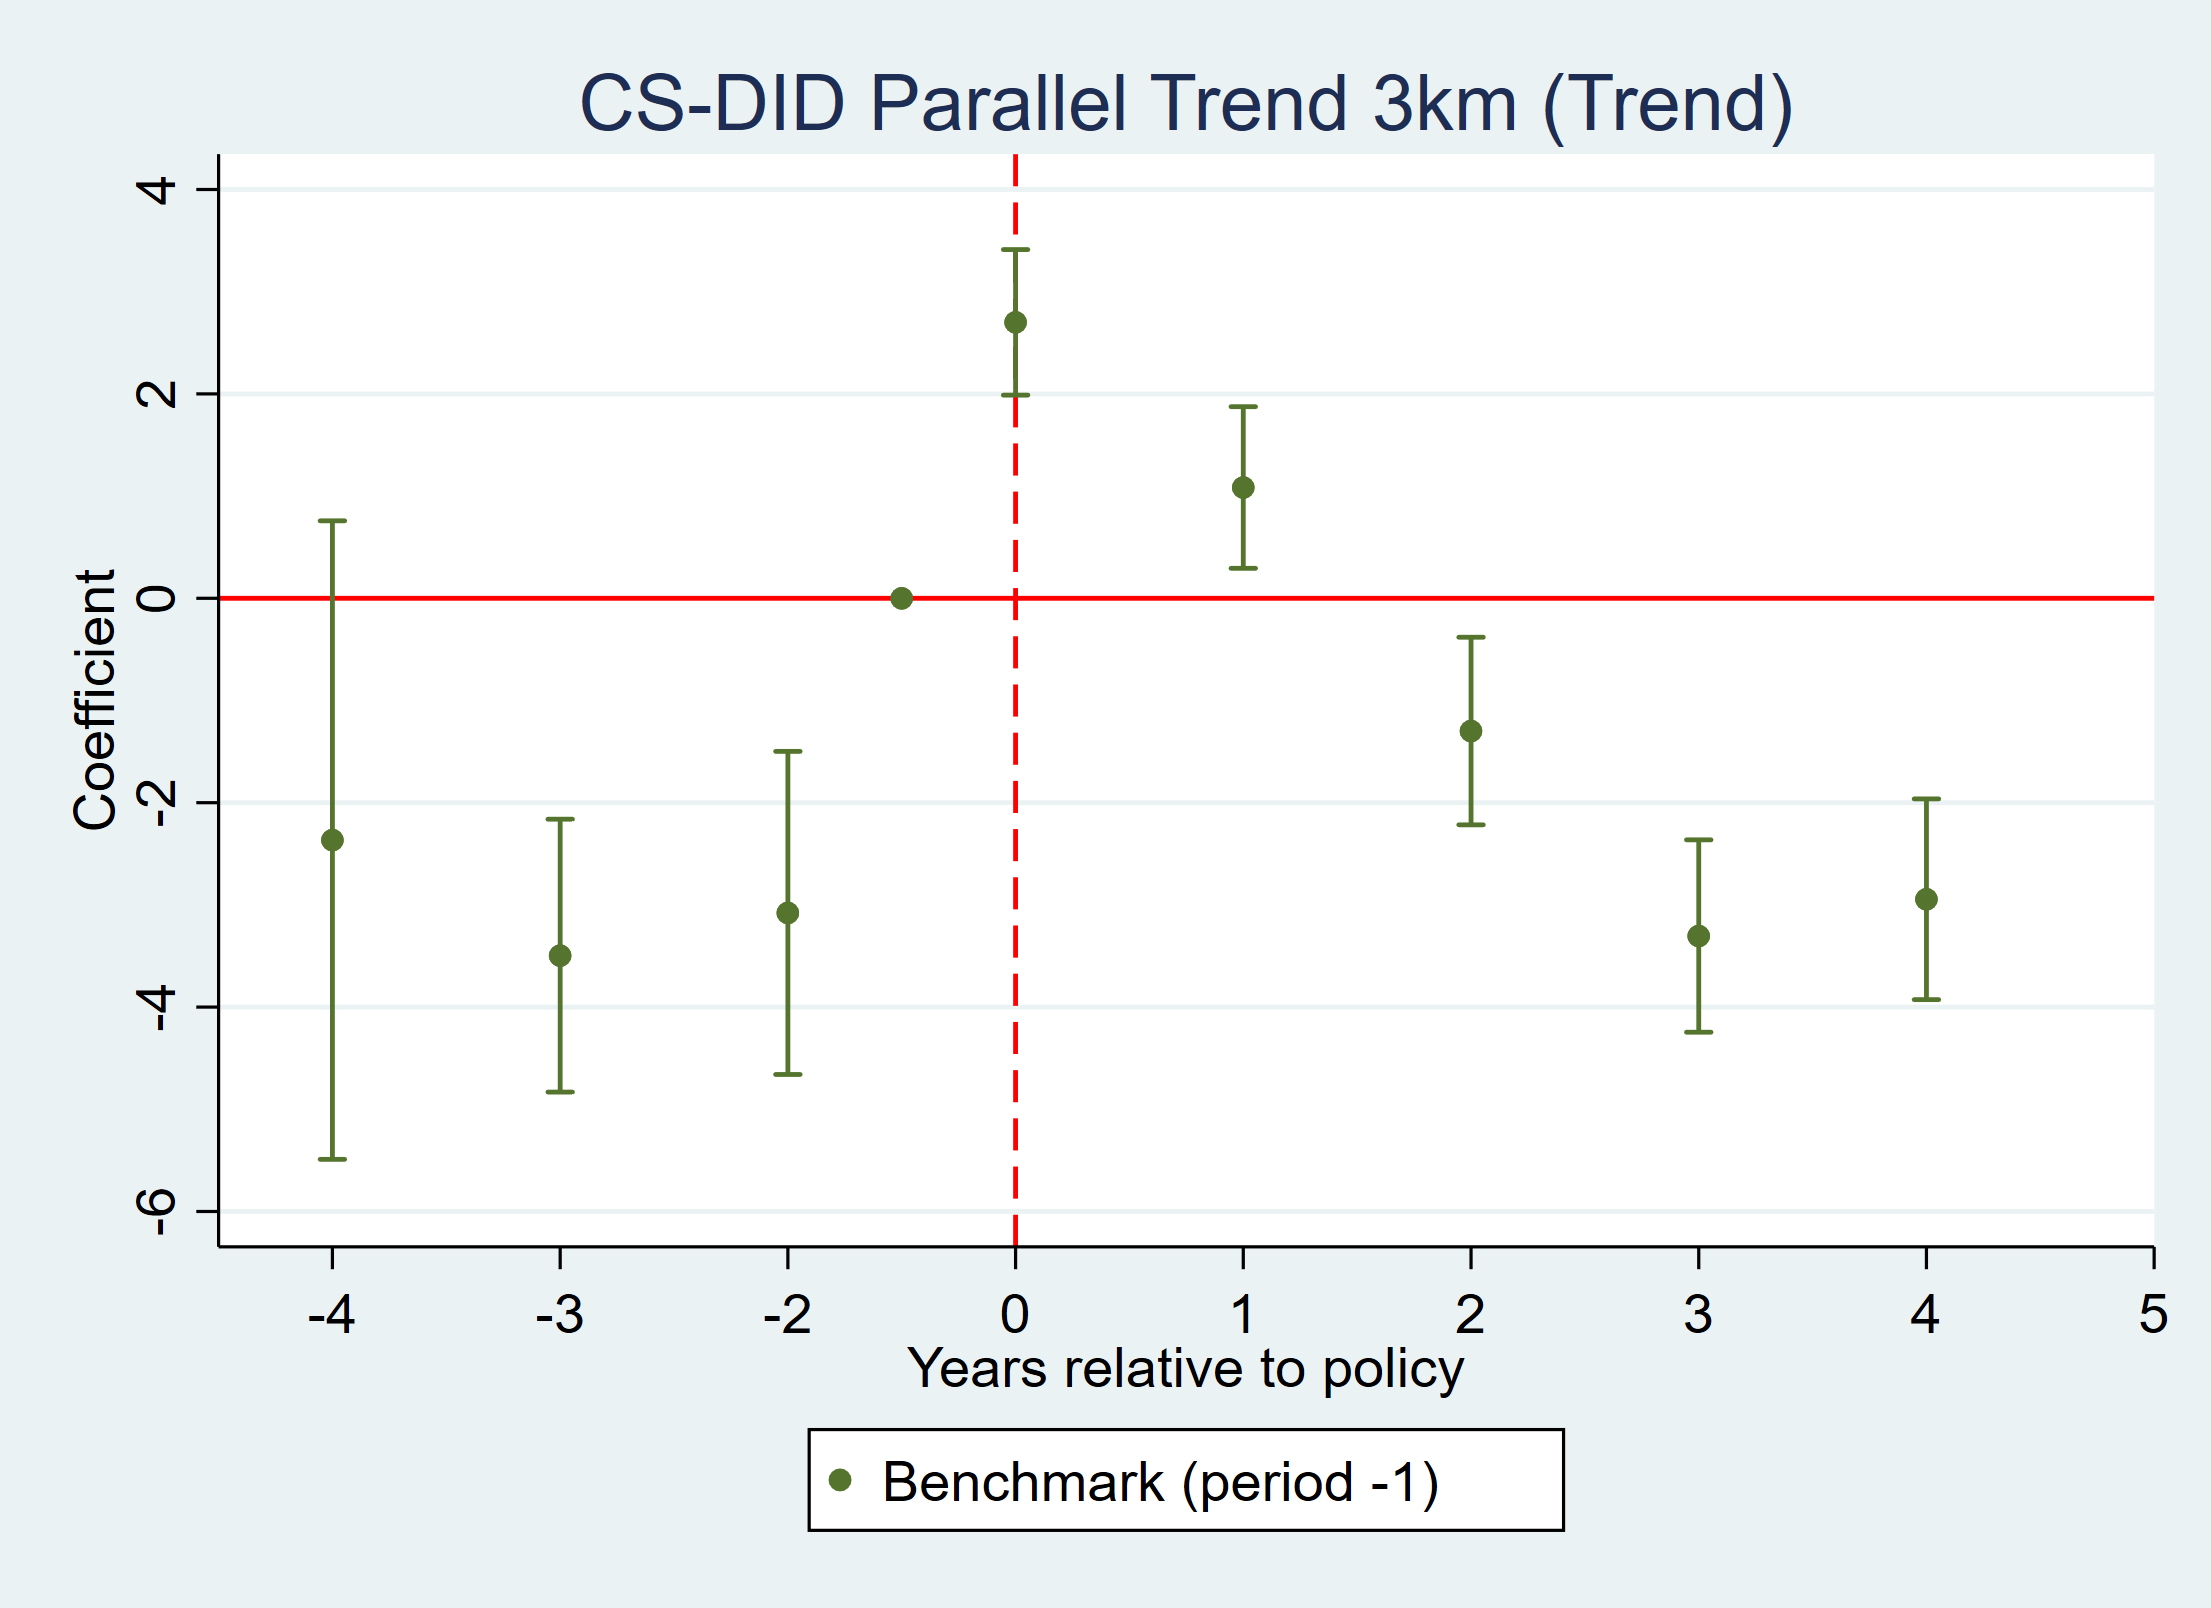
\includegraphics[width=0.8\textwidth]{cs_trend_3km.png}
\end{center}

\end{frame}

% ================= 百分比变化=================
\begin{frame}{Change in Pharmacy Counts Around Treated Hospitals}

\begin{table}[htbp]
\centering
\small
\begin{tabular}{lcccc}
\toprule
\textbf{Radius} & \textbf{Pre-Reform Mean} & \textbf{Post-Reform Mean} & \textbf{Absolute Change} & \textbf{\% Change} \\
\midrule
1km & 7.95 & 11.26 & +3.31 & +41.6\% \\
2km & 23.30 & 30.28 & +6.98 & +30.0\% \\
3km & 41.14 & 50.34 & +9.19 & +22.3\% \\
\bottomrule
\end{tabular}
\end{table}

\vspace{0.3cm}

\textbf{Interpretation}

\begin{itemize}
    \item Pharmacy counts around treated hospitals increased substantially after reform in raw levels.
    \item Growth is strongest within 1km (+41.6\%), suggesting rapid pharmacy expansion near hospitals over time.
    \item However, these are \textbf{before–after comparisons only} and do not net out broader market growth or secular trends.

\end{itemize}


\end{frame}

\begin{frame}{Causal Effect of Reform on Nearby Pharmacy Counts }

\textbf{CS-DID Estimated Treatment Effects }

\begin{table}[htbp]
\centering
\small
\begin{tabular}{lccc}
\toprule
\textbf{Radius} & \textbf{ATE (Level Effect)} & \textbf{Pre-Reform Mean} & \textbf{Percent Effect} \\
\midrule
1km & -0.0736 & 7.95 & -0.93\% \\
2km & -0.3205 & 23.30 & -1.38\% \\
3km & -0.5840 & 41.14 & -1.42\% \\
\bottomrule
\end{tabular}
\end{table}

\vspace{0.3cm}

\textbf{Interpretation}

\begin{itemize}
    \item Although raw before–after counts increased over time, CS-DID suggests this growth was slower than the counterfactual trend.
    \item This implies reform may have weakened hospital-centered pharmacy agglomeration rather than reducing pharmacy growth in absolute terms.
\end{itemize}

\vspace{0.2cm}

\textit{Percent Effect = ATE / Treated Pre-Reform Mean. Negative values indicate fewer pharmacies relative to the treated group’s own baseline.}

\end{frame}


%================= Intensive Margin=================
\begin{frame}{Intensive Margin: OLS}


\textbf{OLS Estimates (Positive-Pharmacy Hospitals Only)}

\begin{table}[htbp]
\centering
\small
\begin{tabular}{lccc}
\toprule
\textbf{Radius} & \textbf{DID Coefficient} & \textbf{Std. Error}  \\
\midrule
1km & +0.457 & (0.242)  \\
2km & +1.615* & (0.707)  \\
3km & +2.955* & (1.315)  \\
\bottomrule
\end{tabular}
\end{table}

\vspace{0.3cm}

\textbf{Interpretation}

\begin{itemize}
    \item Conditional on hospitals already having pharmacy presence, reform is associated with \textbf{higher pharmacy counts}.
    \item Reform may reduce pharmacy entry in marginal/zero-pharmacy areas,
    \item But increase pharmacy concentration in already-developed markets.
\end{itemize}  

\end{frame}

\begin{frame}{Intensive Margin: PPML}

\textbf{PPML Estimates (Positive-Pharmacy Hospitals Only)}

\begin{table}[htbp]
\centering
\small
\begin{tabular}{lccc}
\toprule
\textbf{Radius} & \textbf{PPML Coefficient} & \textbf{Std. Error} \\
\midrule
1km & +0.043** & (0.015) \\
2km & +0.040** & (0.015) \\
3km & +0.036* & (0.016) \\
\bottomrule
\end{tabular}
\end{table}

\vspace{0.3cm}

\textbf{Interpretation}

\begin{itemize}
    \item Among hospitals with sustained positive pharmacy presence, reform increased nearby pharmacy counts on the intensive margin.

    \item Results suggest reform strengthened pharmacy expansion in existing markets rather than reducing incumbent pharmacy activity.
    
    \item Less entry in weak or zero-pharmacy markets,
    \item Greater concentration where pharmacy ecosystems were already established.
    
\end{itemize}

\end{frame}

\begin{frame}{Intensive Margin: Log(1+Y) OLS}

\textbf{Log-OLS Estimates (Positive-Pharmacy Hospitals Only)}

\begin{table}[htbp]
\centering
\small
\begin{tabular}{lccc}
\toprule
\textbf{Radius} & \textbf{Log Coefficient} & \textbf{Std. Error} \\
\midrule
1km & +0.038* & (0.016) \\
2km & +0.049** & (0.017) \\
3km & +0.044* & (0.018) \\
\bottomrule
\end{tabular}
\end{table}

\vspace{0.3cm}

\textbf{Interpretation}

\begin{itemize}

    \item Results closely align with PPML estimates, reinforcing intensive-margin expansion after reform.
    \item Effects are strongest at 2–3km, suggesting pharmacy growth may have shifted outward beyond immediate hospital frontage.

    \item Reduced new entry in weak markets。
    \item Increased pharmacy density in mature local markets.
   
\end{itemize}



\end{frame}

% ================= Mechanism=================
\begin{frame}{Mechanism: Chain Pharmacies(OLS)}

\begin{itemize}
    \item Outcome: Chain pharmacies entry around hospitals 
    \item Fixed effects: hospital and year
    \item Standard errors: clustered at county level
\end{itemize}

\vspace{0.5em}
\centering
\footnotesize
\begin{tabular}{lccc}
\hline
\hline
 & (1) & (2) & (3) \\
 & Chain pharmacy $\sim$1km & Chain pharmacy $\sim$2km & Chain pharmacy $\sim$3km \\
\hline
did & 0.012 & 0.382 & 1.017* \\
    & (0.088) & (0.261) & (0.479) \\
\hline
N   & 188,410 & 188,410 & 188,410 \\
R-sq & 0.682  & 0.719  & 0.733  \\
\hline
\hline
\end{tabular}



\end{frame}


\begin{frame}{Mechanism: Non-Chain Pharmacies}

\begin{itemize}
    \item Outcome: Non-chain pharmacies entry around hospitals 
    \item Fixed effects: hospital and year
    \item Standard errors: clustered at county level
\end{itemize}

\vspace{0.5em}
\centering
\footnotesize
\begin{tabular}{lccc}
\hline
\hline
 & (1) & (2) & (3) \\
 & Non-chain pharmacy $\sim$1km & $\sim$2km & $\sim$3km \\
\hline
did & -0.537*** & -1.553*** & -2.495*** \\
    & (0.117)   & (0.310)   & (0.538)   \\
\hline
N   & 188,410   & 188,410   & 188,410   \\
R-sq & 0.828    & 0.833     & 0.836     \\
\hline
\hline
\end{tabular}


\end{frame}

\begin{frame}{Mechanism: Chain Pharmacies (Share)}

\begin{itemize}
    \item Outcome: Share of chain pharmacies around hospitals 
    \item Fixed effects: hospital and year
    \item Standard errors: clustered at county level
\end{itemize}

\vspace{0.5em}
\centering
\footnotesize
\begin{tabular}{lccc}
\hline
\hline
 & (1) & (2) & (3) \\
 & Chain share $\sim$1km & Chain share $\sim$2km & Chain share $\sim$3km \\
\hline
did & 0.019*** & 0.021*** & 0.022*** \\
    & (0.004)  & (0.004)  & (0.004)  \\
\hline
N   & 159,005  & 170,604  & 174,613  \\
R-sq & 0.788   & 0.840    & 0.851    \\
\hline
\hline
\end{tabular}


\end{frame}

\begin{frame}{Mechanism: Chain Pharmacies (PPML)}

\begin{itemize}
    \item Outcome: Chain pharmacies around hospitals (count)
    \item Estimator: PPML with hospital and year fixed effects
    \item Standard errors: clustered at county level
\end{itemize}

\vspace{0.5em}
\centering
\footnotesize
\begin{tabular}{lccc}
\hline
\hline
 & (1) & (2) & (3) \\
 & Chain pharmacy $\sim$1km & Chain pharmacy $\sim$2km & Chain pharmacy $\sim$3km \\
\hline
did & 0.334*** & 0.353*** & 0.358*** \\
    & (0.088)  & (0.082)  & (0.079)  \\
\hline
N   & 139,926  & 149,752  & 153,318  \\
\hline
\hline
\end{tabular}


\end{frame}

\begin{frame}{Mechanism: Non-chain Pharmacies (PPML)}

\begin{itemize}
    \item Outcome: Non-chain pharmacies around hospitals (count)
    \item Estimator: PPML with hospital and year fixed effects
    \item Standard errors: clustered at county level
\end{itemize}

\vspace{0.5em}
\centering
\footnotesize
\begin{tabular}{lccc}
\hline
\hline
 & (1) & (2) & (3) \\
 & Non-chain $\sim$1km & Non-chain $\sim$2km & Non-chain $\sim$3km \\
\hline
did & 0.007 & 0.010 & 0.016 \\
    & (0.013) & (0.013) & (0.013) \\
\hline
N   & 171,807 & 180,668 & 183,617 \\
\hline
\hline
\end{tabular}
\end{frame}

\begin{frame}{Mechanism: Chain Pharmacies (Share, PPML)}

\begin{itemize}
    \item Outcome: Share of chain pharmacies around hospitals
    \item Estimator: PPML with hospital and year fixed effects
    \item Standard errors: clustered at county level
\end{itemize}

\vspace{0.5em}
\centering
\footnotesize
\begin{tabular}{lccc}
\hline
\hline
 & (1) & (2) & (3) \\
 & Chain share $\sim$1km & Chain share $\sim$2km & Chain share $\sim$3km \\
\hline
did & 0.205*** & 0.229*** & 0.242*** \\
    & (0.061)  & (0.057)  & (0.057)  \\
\hline
N   & 129,869  & 141,824  & 146,097  \\
\hline
\hline
\end{tabular}

\end{frame}
% ================= Summary =================
\begin{frame}{Summary}

\begin{itemize}
    \item DID: OLS negative and significant ,CS  negative but insignificant ,PPML positive and significant 
    \item Event Study: PPML, supporting causal inference
    \item  How to adjust event study 
\end{itemize}

\vspace{0.6cm}

\centering
\textbf{The reform increases pharmacy entry around hospitals}

\end{frame}

\end{document}